% Options for packages loaded elsewhere
\PassOptionsToPackage{unicode}{hyperref}
\PassOptionsToPackage{hyphens}{url}
%
\documentclass[
]{article}
\usepackage{lmodern}
\usepackage{amsmath}
\usepackage{ifxetex,ifluatex}
\ifnum 0\ifxetex 1\fi\ifluatex 1\fi=0 % if pdftex
  \usepackage[T1]{fontenc}
  \usepackage[utf8]{inputenc}
  \usepackage{textcomp} % provide euro and other symbols
  \usepackage{amssymb}
\else % if luatex or xetex
  \usepackage{unicode-math}
  \defaultfontfeatures{Scale=MatchLowercase}
  \defaultfontfeatures[\rmfamily]{Ligatures=TeX,Scale=1}
\fi
% Use upquote if available, for straight quotes in verbatim environments
\IfFileExists{upquote.sty}{\usepackage{upquote}}{}
\IfFileExists{microtype.sty}{% use microtype if available
  \usepackage[]{microtype}
  \UseMicrotypeSet[protrusion]{basicmath} % disable protrusion for tt fonts
}{}
\makeatletter
\@ifundefined{KOMAClassName}{% if non-KOMA class
  \IfFileExists{parskip.sty}{%
    \usepackage{parskip}
  }{% else
    \setlength{\parindent}{0pt}
    \setlength{\parskip}{6pt plus 2pt minus 1pt}}
}{% if KOMA class
  \KOMAoptions{parskip=half}}
\makeatother
\usepackage{xcolor}
\IfFileExists{xurl.sty}{\usepackage{xurl}}{} % add URL line breaks if available
\IfFileExists{bookmark.sty}{\usepackage{bookmark}}{\usepackage{hyperref}}
\hypersetup{
  pdftitle={Checkmate 067 study Bayesian mixture cure model analysis},
  pdfauthor={Nathan Green, Gianluca Baio, UCL},
  hidelinks,
  pdfcreator={LaTeX via pandoc}}
\urlstyle{same} % disable monospaced font for URLs
\usepackage[margin=1in]{geometry}
\usepackage{longtable,booktabs}
% Correct order of tables after \paragraph or \subparagraph
\usepackage{etoolbox}
\makeatletter
\patchcmd\longtable{\par}{\if@noskipsec\mbox{}\fi\par}{}{}
\makeatother
% Allow footnotes in longtable head/foot
\IfFileExists{footnotehyper.sty}{\usepackage{footnotehyper}}{\usepackage{footnote}}
\makesavenoteenv{longtable}
\usepackage{graphicx}
\makeatletter
\def\maxwidth{\ifdim\Gin@nat@width>\linewidth\linewidth\else\Gin@nat@width\fi}
\def\maxheight{\ifdim\Gin@nat@height>\textheight\textheight\else\Gin@nat@height\fi}
\makeatother
% Scale images if necessary, so that they will not overflow the page
% margins by default, and it is still possible to overwrite the defaults
% using explicit options in \includegraphics[width, height, ...]{}
\setkeys{Gin}{width=\maxwidth,height=\maxheight,keepaspectratio}
% Set default figure placement to htbp
\makeatletter
\def\fps@figure{htbp}
\makeatother
\setlength{\emergencystretch}{3em} % prevent overfull lines
\providecommand{\tightlist}{%
  \setlength{\itemsep}{0pt}\setlength{\parskip}{0pt}}
\setcounter{secnumdepth}{-\maxdimen} % remove section numbering
\ifluatex
  \usepackage{selnolig}  % disable illegal ligatures
\fi
\newlength{\cslhangindent}
\setlength{\cslhangindent}{1.5em}
\newlength{\csllabelwidth}
\setlength{\csllabelwidth}{3em}
\newenvironment{CSLReferences}[3] % #1 hanging-ident, #2 entry spacing
 {% don't indent paragraphs
  \setlength{\parindent}{0pt}
  % turn on hanging indent if param 1 is 1
  \ifodd #1 \everypar{\setlength{\hangindent}{\cslhangindent}}\ignorespaces\fi
  % set entry spacing
  \ifnum #2 > 0
  \setlength{\parskip}{#2\baselineskip}
  \fi
 }%
 {}
\usepackage{calc} % for \widthof, \maxof
\newcommand{\CSLBlock}[1]{#1\hfill\break}
\newcommand{\CSLLeftMargin}[1]{\parbox[t]{\maxof{\widthof{#1}}{\csllabelwidth}}{#1}}
\newcommand{\CSLRightInline}[1]{\parbox[t]{\linewidth}{#1}}
\newcommand{\CSLIndent}[1]{\hspace{\cslhangindent}#1}

\title{Checkmate 067 study Bayesian mixture cure model analysis}
\author{Nathan Green, Gianluca Baio, UCL}
\date{30 March, 2021}

\begin{document}
\maketitle

\hypertarget{executive-summary}{%
\subsubsection{Executive summary}\label{executive-summary}}

In this project we formulate and demonstrate the application of a
Bayesian mixture cure model (MCM) using the Checkmate 067 study dataset
for a range of survival distributions. Analogous results to those
created previously for the frequentist MCM approach are produced and we
extend the Bayesian MCM to incorporate additional structure. This
includes modelling the cure fractions separately for OS and PFS (as in
the frequentist approach) and by joining the overall survival (OS) and
progression-free survival (PFS) models using a hierarchical (multilevel)
structure on the cure fraction. We show that the Exponential and in
particular the log-logistic OS and PFS Bayesian MCMs perform reasonably
well for the Checkmate 067 data. We also perform a sensitivity analysis
by increasing the background hazard rate via a hazard ratio adjustment,
representing a study population with a higher mortality rate than the
general population. The real benefit of this approach, not full explored
in this analysis, may be with other dataset where there is relatively
short follow-up or small sample sizes. The associated R code for this
work, held in a private on-line repository, has been written for re-use
and generalisability to other problems.

\hypertarget{background}{%
\subsection{Background}\label{background}}

Immuno-oncologic (IO) studies for melanoma therapies, such as
\emph{ipilimumab} (\texttt{ipi}), \emph{nivolumab} (\texttt{nivo}), and
the \emph{nivolumab} with \emph{ipilimumab} (\texttt{nivo\ +\ ipi})
combination, have indicated that survival curves ``plateau'' (a
considerable proportion of patients are ``long-term survivors''). Cure
models are a special type of survival analysis where this ``cure
fraction'' (the underlying proportion of responders to
treatment/long-term survivors) is accounted for. Cure models estimate
the cure fraction, in addition to a parametric survival function for
patients that are not cured. The mortality risk in the cured patients is
informed by a background mortality rate. The population that is not
cured is subject both to background mortality and to additional
mortality from their cancer, estimated using a parametric survival
model.

A mixture cure model (MCM) (Amico and Van Keilegom (2018)) is a type of
cure model where survival is modelled as a mixture of two groups of
patients: those who are cured and those who are not (and who therefore
remain at risk). The survival for a population with a cure fraction can
be written as follows:

\begin{align}
\tag{*}
S(t, x) = S^*(t, x)[\pi(x) + (1 − \pi(x))S_u(t, x)],
\end{align}

where \(S(t, x)\) denotes the survival at time \(t\), \(S^*(t, x)\)
denotes the background mortality at time \(t\) conditional on covariates
\(x\), \(\pi(x)\) denotes the probability of being cured conditional on
covariates \(x\), and \(S_u(t, x)\) denotes the event (progression or
mortality) due to cancer at time \(t\) conditional on covariates \(x\).
For PFS, the survival is composed of either progressing to a disease
state or death.

\hypertarget{aims}{%
\subsection{Aims}\label{aims}}

The aims of the the analysis in this document are as follows:

\begin{itemize}
\tightlist
\item
  Demonstrate the application of a Bayesian mixture cure model using the
  Checkmate 067 study dataset and the Exponential distribution for event
  times.
\item
  Produce analogous results to those created previously for the
  frequentist approach.
\item
  Extend the Bayesian model to incorporate additional structure
  including a hierarchical cure fraction.
\end{itemize}

This analysis has been carried-out using the Stan inference engine
(Carpenter et al. (2017)) called from R on a Windows PC. The packaged
code can be downloaded from a private GitHub repository with permission
from the package authors at
\url{https://github.com/StatisticsHealthEconomics/rstanbmcm}. See the
\emph{How to use rstanbmcm} vignette for an introduction to how to use
the package.

\hypertarget{likelihood}{%
\subsection{Likelihood}\label{likelihood}}

Let \(T_i\) be the non-negative random variable denoting the survival
time of patient \(i\) with covariate vector \(\boldsymbol{x}_i\).

In the simplest case we can assume that the cure fraction is the same
for the whole population i.e.~\(\pi\) is fixed. Further, we can assume
the \(\pi\) models the relationship between \(\boldsymbol{x}_i\) and the
probability of being cured. E.g. using a logistic-linear model

\[
\pi(\boldsymbol{x}_i | \boldsymbol{\beta}) = 1/[1 + \exp(-\boldsymbol{x}_i^T \boldsymbol{\beta})].
\]

The likelihood of the standard survival is

\[
L = \prod_i S(t_i | \boldsymbol{x}_i) h(t_i | \boldsymbol{x}_i)^{\delta_i}
\]

Log-likelihood is therefore \[
\mathcal{l} = \sum_i \log(S(t_i | \boldsymbol{x}_i)) + \delta_i \log(h(t_i | \boldsymbol{x}_i))
\]

Plugging this directly into the mixture cure equation in (*) gives

\[
\mathcal{l}(\pi | \boldsymbol{\delta}, \boldsymbol{x}) =
 \sum_i \log(S^*(t_i | \boldsymbol{x}_i) h^*(t_i | \boldsymbol{x}_i)^{\delta_i}[\pi(x) +
   (1 − \pi(x)) S_u(t_i | \boldsymbol{x}_i) h_u(t_i | \boldsymbol{x}_i)^{\delta_i}])
\]

If we assume that the cured component is the Exponential survival model
then the non-cured component can be thought of in similar terms to the
cumulative incidence function. That is, the probability of an event is
the combined probability of surviving both events (e.g.~for OS,
all-cause and cancer mortality) and then experiencing either i.e.
dropping the \(S\) dependencies for brevity

\begin{equation}
\tag{**}
S^* S_u (h^*)^{\delta} + S^* S_u (h_u)^{\delta} = S^* S_u (h^* + h_u)^{\delta}
\end{equation}

\hypertarget{bayesian-formulation}{%
\subsection{Bayesian formulation}\label{bayesian-formulation}}

In a Bayesian approach to modelling (McElreath (2018)), all quantities
that are subject to uncertainty are modelled using probability
distributions. This applies to observed data (e.g.~time to PFS for a
given individual), that are subject to sampling variability, as well as
to unobservable parameters (e.g.~the coefficient quantifying the impact
of age or sex over the average survival curve). In this latter case,
probability distributions are used to model the epistemic uncertainty
(e.g.~the fact that we do not know for certain what the ``true''
underlying value of the model parameter is). In addition, we may model
as yet unobserved (but potentially observable) quantities using a
suitable probability model. For example, we could consider the
extrapolated part of the survival curve as subject to uncertainty due to
the current sampling process giving rise to the data that are actually
observed, as well as the uncertainty on the underlying data generating
process.

We can mix different sources of evidence to form our ``prior''
distributions, which are used to describe the state of science on the
model parameters. These are then combined with any observed data to form
an updated level of knowledge. This process is particularly relevant in
the case at hand, when data can only inform about limited aspects of the
overall underlying reality. For this reason, it is important to a)
include information/evidence available in the form of external data
and/or expert opinion; b) extract the most information possible from the
available data (e.g.~by formally trying to model the correlation between
the PFS and the OS data to borrow strength from the more mature set of
observations).

A built-in advantage of the Bayesian procedure is that uncertainty is
directly and formally propagated to an economic model; the main output
from the statistical analysis (the extrapolated survival curve) are
produced by default as based on a full posterior distribution. From
this, we can easily derive a ``base case'' (e.g.~taking the mean value)
but without the need for further tools (such as bootstrap) we already
have a full characterisation of the underlying uncertainty that can be
used in the process of probabilistic sensitivity analysis. We can
moreover add information in the priors to ensure that the extrapolation
beyond the observed data is realistic and consistent with the clinical
expertise (e.g.~by ``anchoring'' the extrapolated survival curve to be
probabilistically below the curves for the healthy population, or by
ensuring that OS behaves in a way to respect some agreed level of
similarity, or correlation, to PFS).

\hypertarget{posterior-equation}{%
\paragraph{Posterior equation}\label{posterior-equation}}

Using the likelihood function defined above and prior distributions on
uncertain parameters, we can specify the posterior distribution.
Defining \(g_2\) as the prior distribution for the coefficients of the
uncured fraction \(\beta^u\) and \(g_3\) as the prior distribution for
the coefficients of the cured fraction \(\beta^*\), then the general
form of the posterior distribution can be written as follows.

\[
p(\pi, \boldsymbol{\beta^u}, \boldsymbol{\beta^*} | \boldsymbol{\delta}, \boldsymbol{x}) \propto
L(\pi, \boldsymbol{\beta^u}, \boldsymbol{\beta^*} | \boldsymbol{\delta}, \boldsymbol{x}) f(\pi) g_2(\boldsymbol{\beta^u}) g_3(\boldsymbol{\beta^*})
\]

assuming that the cure fraction is independent of the covariates.

\hypertarget{cure-fraction}{%
\subsubsection{Cure fraction}\label{cure-fraction}}

There are two obvious ways to represent the uncertainty about the cure
fraction in the model.

The first is to specify the cure fraction directly using a
\(\pi \sim Beta(a_{cf}, b_{cf})\) prior, most uninformative as a uniform
\(Beta(1,1)\). The parameters can be obtained via transformation of mean
and standard deviation to allow a more natural scale for elicitation.

Alternatively, we may specify the uncertainty on the real line with a
Normal distribution and then transform to the probability scale.

A further consideration is how to represent the cure fraction so to
share information between the OS and PFS data. We will investigate 3
alternatives.

\begin{itemize}
\tightlist
\item
  \emph{Pooled}: Assume that the cure fraction is the same for OS and
  PFS i.e.~\(\pi_{os} = \pi_{os} = \pi\) where \[
  logit(\pi) \sim N(\mu_{cf}, \sigma_{cf}^2), \;\;
  \]
\item
  \emph{Separate}: Model each independently. \[
  logit(\pi_{os}) \sim N(\mu_{cfos}, \sigma_{cfos}^2), \;\;  
  logit(\pi_{pfs}) \sim N(\mu_{cfpfs}, \sigma_{cfpfs}^2)  
  \]
\item
  \emph{Hierarchical}: Assume exchangeability between OS and PFS\[
  \pi \sim N(\mu_{cf}, \sigma_{cf}^2), \;\;  
  logit(\pi_{os}) \sim N(\pi, \sigma_{cfos}^2), \;\;  
  logit(\pi_{pfs}) \sim N(\pi, \sigma_{cfpfs}^2)  
  \]
\end{itemize}

Below is an example DAG for the hierarchical cure fraction without a
joint time to event component. Notice that even without the direct
relationship between PFS and OS there is still an indirect influence via
\(\pi\).

\begin{figure}

{\centering 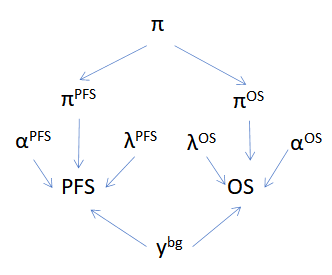
\includegraphics[width=0.4\linewidth]{hierarchical_DAG} 

}

\caption{\label{fig:hier_dag} Hierarchical cure fraction DAG.}\label{fig:unnamed-chunk-2}
\end{figure}

\hypertarget{background-survival}{%
\subsection{Background survival}\label{background-survival}}

The previous frequentist analysis used the World Health Organization
(WHO) life tables by country for the latest year available of 2016 (WHO
(2020)) to inform the background mortality rate (baseline hazard). These
baseline hazards are the expected mortality rate for each patient at the
age at which they experience the event. The mortality data are age- and
gender adjusted, thus providing a granular account of the different
patient profiles in the trial. The WHO reports conditional probabilities
of death in 5-year intervals until age 85. A constant annual mortality
rate is reported for individuals over 85. They assumed that the maximum
age is 100 years.

In a Bayesian analysis there are alternative ways in which we could
model the background mortality.

For this work we shall use WHO hazard point estimates as known. We could
consider the WHO estimates to provide sufficiently accurate estimates
given the sample size and so incorporating uncertainty is not necessary.
This also forces consistency across fits. Denote the WHO estimates for
individual \(i\) as \(\hat{f}_i, \hat{S}_i, \hat{h}_i\) for the density,
survival and hazard respectively.

This gives the likelihood

\[
L(\pi | \boldsymbol{\delta}, \boldsymbol{x}, \hat{S}, \hat{h}) =
\sum_i \hat{S}_i \hat{h}_i^{\delta_i} \left[ \pi(x) + (1 - \pi(x)) S_{u, i} h_{u , i}^{\delta_i} \right]
\]

\hypertarget{results}{%
\subsection{Results}\label{results}}

We fit the separate and exchangeable cure fraction models to the study
data and produced the posterior survival curves below.

For each model and treatment we produce the expected survival curves
with 95\% Credible Intervals (CrI). The OS curves are to the left-hand
side and PFS curves to the right-hand side. Background mortality
(i.e.~cured patients) is indicated by the red line. Non-cured patients
survival curves are shown in dark green and blue for OS and PFS
respectively. Light green and magenta are the total sample. The black
line is the Kaplan-Meier curve for the observed data. Note that these
plots are for an average individual, e.g.~at average age, and so we
would not expect them to perfectly match the sample data Kaplan-Meier.

\hypertarget{separate-survival-models-for-os-and-pfs}{%
\subsubsection{Separate survival models for OS and
PFS}\label{separate-survival-models-for-os-and-pfs}}

Figures \ref{fig:IPI_separate}, \ref{fig:NIVO_separate}, and
\ref{fig:NIVO+IPI_separate} show posterior survival curves for the
Exponential, log-logistic, Gompertz, Weibull and log-Normal models when
the OS and PFS models are fitted separately.

\begin{figure}

{\centering 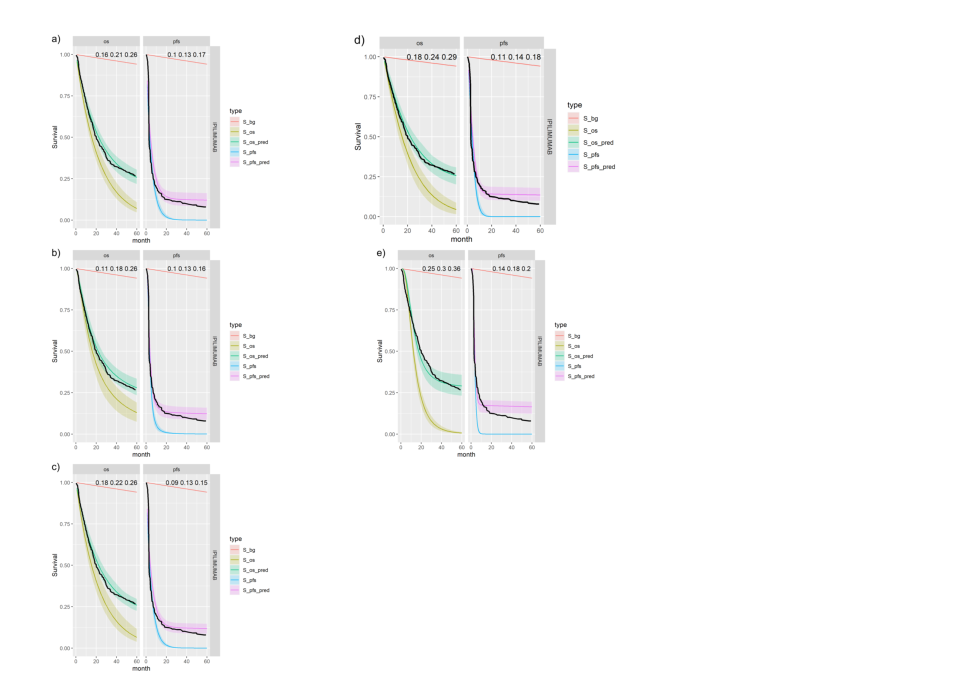
\includegraphics[width=25cm,height=40cm]{Check_mate_analysis_files/figure-latex/unnamed-chunk-3-1} 

}

\caption{\label{fig:IPI_separate}Posterior survival curves for the mixture cure model for separate OS and PFS models and $ipilimumab$. The red line is cured background, light green and blue are uncured, and dark green and magenta are combined. a) Exponential uncured b) Log-logistic uncured c) Gompertz uncured d) Weibull uncured e) Log-Normal uncured.}\label{fig:unnamed-chunk-3}
\end{figure}

\begin{figure}

{\centering 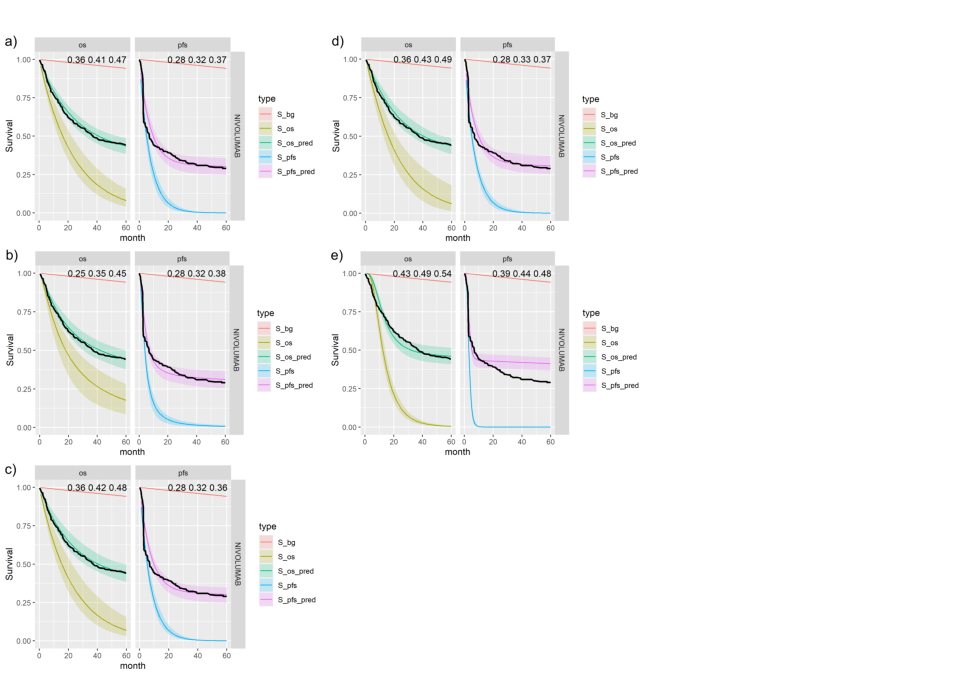
\includegraphics[width=25cm,height=40cm]{Check_mate_analysis_files/figure-latex/unnamed-chunk-4-1} 

}

\caption{\label{fig:NIVO_separate}Posterior survival curves for the mixture cure model for separate OS and PFS models and $nivolumab$. The red line is cured background, light green and blue are uncured, and dark green and magenta are combined. a) Exponential uncured b) Log-logistic uncured c) Gompertz uncured d) Weibull uncured e) Log-Normal uncured.}\label{fig:unnamed-chunk-4}
\end{figure}

\begin{figure}

{\centering 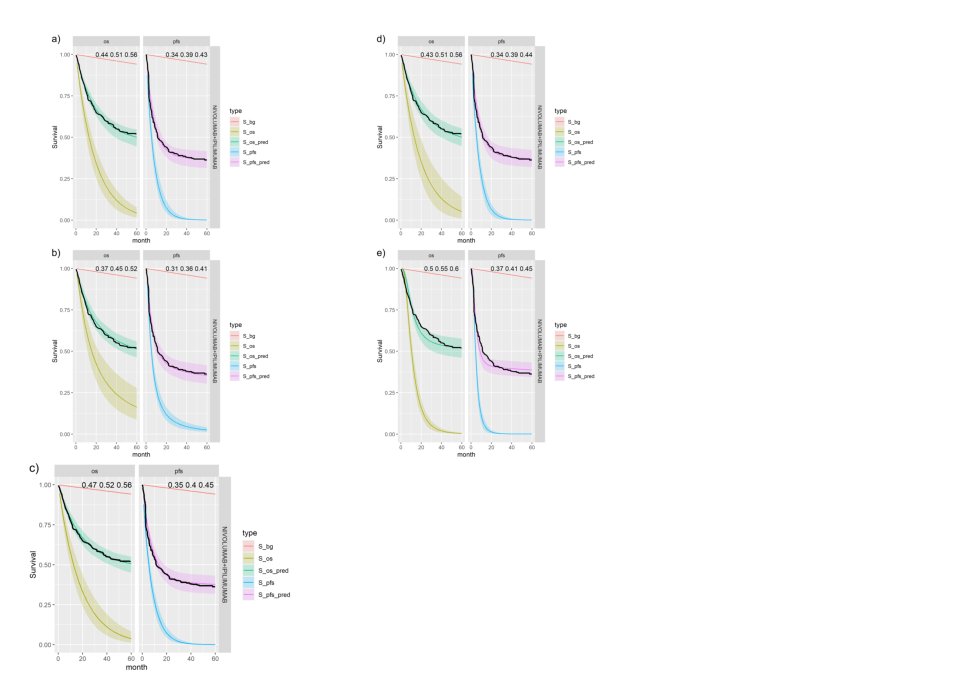
\includegraphics[width=25cm,height=40cm]{Check_mate_analysis_files/figure-latex/unnamed-chunk-5-1} 

}

\caption{\label{fig:NIVO+IPI_separate}Posterior survival curves for the mixture cure model for separate OS and PFS models and $ipilimumab$ and $nivolumab$. The red line is cured background, light green and blue are uncured, and dark green and magenta are combined. a) Exponential uncured b) Log-logistic uncured c) Gompertz uncured d) Weibull uncured e) Log-Normal uncured.}\label{fig:unnamed-chunk-5}
\end{figure}

Figures \ref{fig:forest_os_separate} and \ref{fig:forest_pfs_separate}
show the forest plots of cure fraction posterior distributions.

\begin{figure}

{\centering 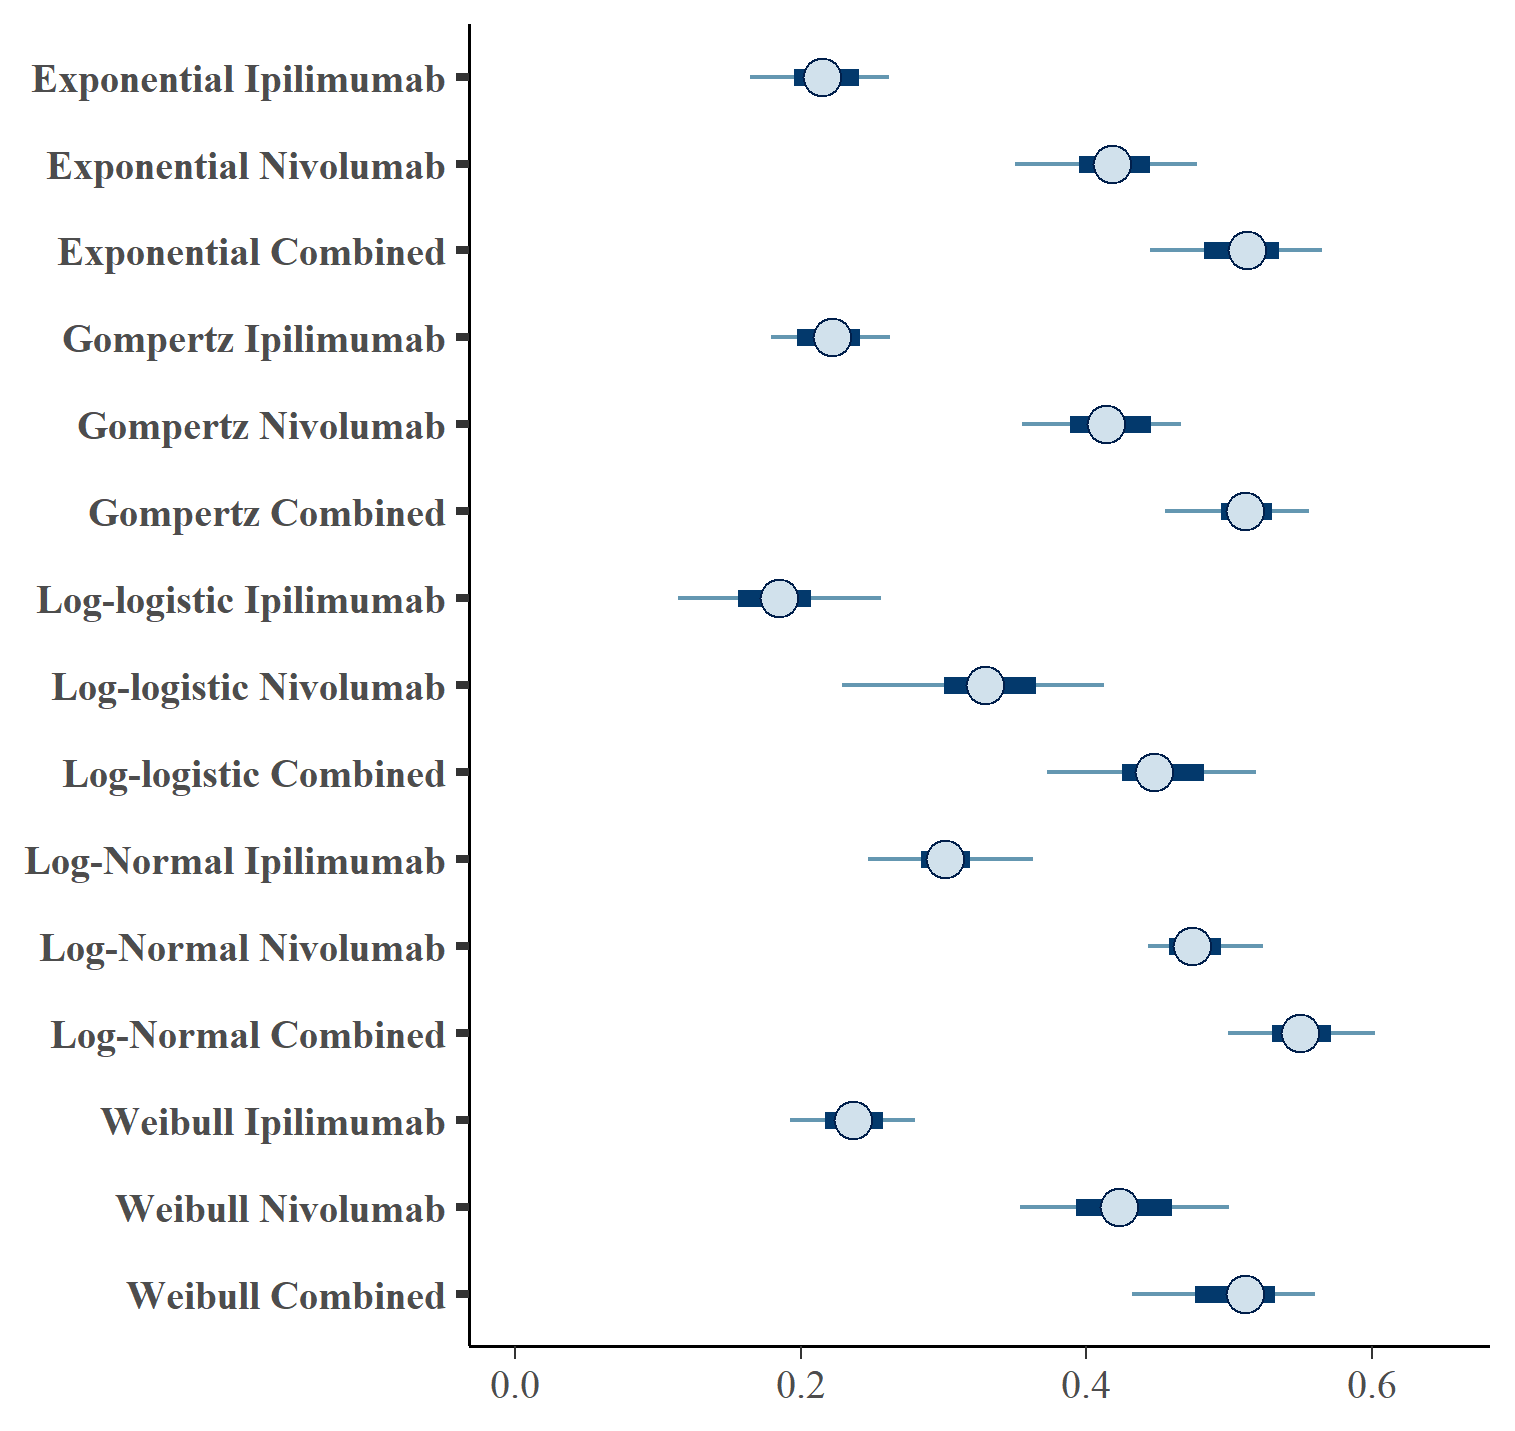
\includegraphics[width=0.6\linewidth]{../plots/cf separate_os_forest_plot} 

}

\caption{\label{fig:forest_os_separate}Forest plot of OS cure fraction posterior distributions for separate OS and PFS models .}\label{fig:unnamed-chunk-6}
\end{figure}

\begin{figure}

{\centering 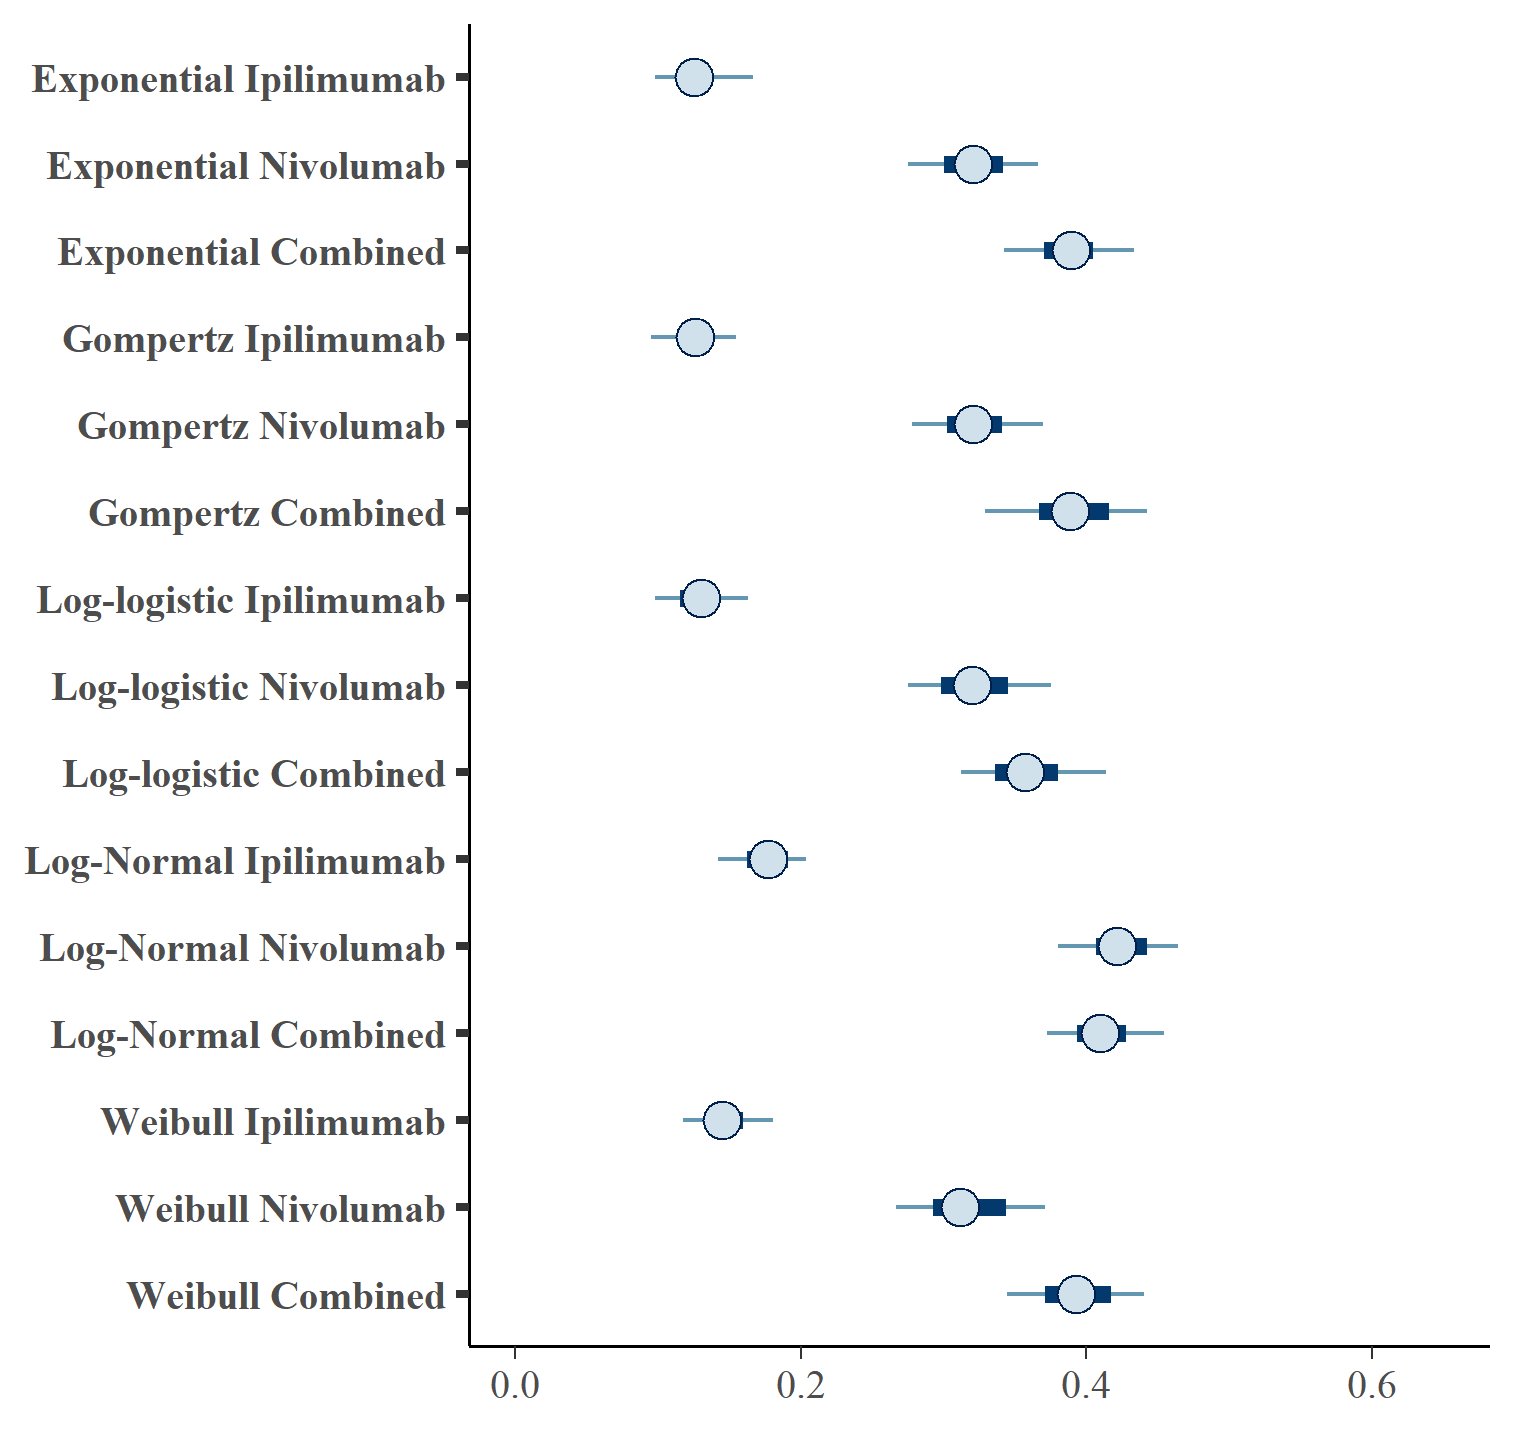
\includegraphics[width=0.6\linewidth]{../plots/cf separate_pfs_forest_plot} 

}

\caption{\label{fig:forest_pfs_separate}Forest plot of PFS cure fraction posterior distributions for separate OS and PFS models .}\label{fig:unnamed-chunk-7}
\end{figure}

\begin{longtable}[]{@{}llllll@{}}
\toprule
\begin{minipage}[b]{0.03\columnwidth}\raggedright
\strut
\end{minipage} & \begin{minipage}[b]{0.11\columnwidth}\raggedright
OS Distn\strut
\end{minipage} & \begin{minipage}[b]{0.11\columnwidth}\raggedright
PFS Distn\strut
\end{minipage} & \begin{minipage}[b]{0.19\columnwidth}\raggedright
Treatment\strut
\end{minipage} & \begin{minipage}[b]{0.19\columnwidth}\raggedright
\(cf_{OS}\) (CrI)\strut
\end{minipage} & \begin{minipage}[b]{0.19\columnwidth}\raggedright
\(cf_{PFS}\) (CrI)\strut
\end{minipage}\tabularnewline
\midrule
\endhead
\begin{minipage}[t]{0.03\columnwidth}\raggedright
1\strut
\end{minipage} & \begin{minipage}[t]{0.11\columnwidth}\raggedright
exp\strut
\end{minipage} & \begin{minipage}[t]{0.11\columnwidth}\raggedright
exp\strut
\end{minipage} & \begin{minipage}[t]{0.19\columnwidth}\raggedright
IPILIMUMAB\strut
\end{minipage} & \begin{minipage}[t]{0.19\columnwidth}\raggedright
0.216 (0.16, 0.271)\strut
\end{minipage} & \begin{minipage}[t]{0.19\columnwidth}\raggedright
0.128 (0.089, 0.173)\strut
\end{minipage}\tabularnewline
\begin{minipage}[t]{0.03\columnwidth}\raggedright
2\strut
\end{minipage} & \begin{minipage}[t]{0.11\columnwidth}\raggedright
exp\strut
\end{minipage} & \begin{minipage}[t]{0.11\columnwidth}\raggedright
exp\strut
\end{minipage} & \begin{minipage}[t]{0.19\columnwidth}\raggedright
NIVOLUMAB\strut
\end{minipage} & \begin{minipage}[t]{0.19\columnwidth}\raggedright
0.417 (0.335, 0.482)\strut
\end{minipage} & \begin{minipage}[t]{0.19\columnwidth}\raggedright
0.32 (0.268, 0.37)\strut
\end{minipage}\tabularnewline
\begin{minipage}[t]{0.03\columnwidth}\raggedright
3\strut
\end{minipage} & \begin{minipage}[t]{0.11\columnwidth}\raggedright
exp\strut
\end{minipage} & \begin{minipage}[t]{0.11\columnwidth}\raggedright
exp\strut
\end{minipage} & \begin{minipage}[t]{0.19\columnwidth}\raggedright
NIVOLUMAB+IPILIMUMAB\strut
\end{minipage} & \begin{minipage}[t]{0.19\columnwidth}\raggedright
0.509 (0.43, 0.573)\strut
\end{minipage} & \begin{minipage}[t]{0.19\columnwidth}\raggedright
0.387 (0.332, 0.441)\strut
\end{minipage}\tabularnewline
\begin{minipage}[t]{0.03\columnwidth}\raggedright
4\strut
\end{minipage} & \begin{minipage}[t]{0.11\columnwidth}\raggedright
gompertz\strut
\end{minipage} & \begin{minipage}[t]{0.11\columnwidth}\raggedright
gompertz\strut
\end{minipage} & \begin{minipage}[t]{0.19\columnwidth}\raggedright
IPILIMUMAB\strut
\end{minipage} & \begin{minipage}[t]{0.19\columnwidth}\raggedright
0.221 (0.176, 0.282)\strut
\end{minipage} & \begin{minipage}[t]{0.19\columnwidth}\raggedright
0.126 (0.092, 0.156)\strut
\end{minipage}\tabularnewline
\begin{minipage}[t]{0.03\columnwidth}\raggedright
5\strut
\end{minipage} & \begin{minipage}[t]{0.11\columnwidth}\raggedright
gompertz\strut
\end{minipage} & \begin{minipage}[t]{0.11\columnwidth}\raggedright
gompertz\strut
\end{minipage} & \begin{minipage}[t]{0.19\columnwidth}\raggedright
NIVOLUMAB\strut
\end{minipage} & \begin{minipage}[t]{0.19\columnwidth}\raggedright
0.414 (0.352, 0.477)\strut
\end{minipage} & \begin{minipage}[t]{0.19\columnwidth}\raggedright
0.321 (0.274, 0.383)\strut
\end{minipage}\tabularnewline
\begin{minipage}[t]{0.03\columnwidth}\raggedright
6\strut
\end{minipage} & \begin{minipage}[t]{0.11\columnwidth}\raggedright
gompertz\strut
\end{minipage} & \begin{minipage}[t]{0.11\columnwidth}\raggedright
gompertz\strut
\end{minipage} & \begin{minipage}[t]{0.19\columnwidth}\raggedright
NIVOLUMAB+IPILIMUMAB\strut
\end{minipage} & \begin{minipage}[t]{0.19\columnwidth}\raggedright
0.51 (0.447, 0.575)\strut
\end{minipage} & \begin{minipage}[t]{0.19\columnwidth}\raggedright
0.39 (0.323, 0.457)\strut
\end{minipage}\tabularnewline
\begin{minipage}[t]{0.03\columnwidth}\raggedright
7\strut
\end{minipage} & \begin{minipage}[t]{0.11\columnwidth}\raggedright
loglogistic\strut
\end{minipage} & \begin{minipage}[t]{0.11\columnwidth}\raggedright
loglogistic\strut
\end{minipage} & \begin{minipage}[t]{0.19\columnwidth}\raggedright
IPILIMUMAB\strut
\end{minipage} & \begin{minipage}[t]{0.19\columnwidth}\raggedright
0.183 (0.11, 0.265)\strut
\end{minipage} & \begin{minipage}[t]{0.19\columnwidth}\raggedright
0.13 (0.091, 0.168)\strut
\end{minipage}\tabularnewline
\begin{minipage}[t]{0.03\columnwidth}\raggedright
8\strut
\end{minipage} & \begin{minipage}[t]{0.11\columnwidth}\raggedright
loglogistic\strut
\end{minipage} & \begin{minipage}[t]{0.11\columnwidth}\raggedright
loglogistic\strut
\end{minipage} & \begin{minipage}[t]{0.19\columnwidth}\raggedright
NIVOLUMAB\strut
\end{minipage} & \begin{minipage}[t]{0.19\columnwidth}\raggedright
0.329 (0.217, 0.423)\strut
\end{minipage} & \begin{minipage}[t]{0.19\columnwidth}\raggedright
0.321 (0.267, 0.381)\strut
\end{minipage}\tabularnewline
\begin{minipage}[t]{0.03\columnwidth}\raggedright
9\strut
\end{minipage} & \begin{minipage}[t]{0.11\columnwidth}\raggedright
loglogistic\strut
\end{minipage} & \begin{minipage}[t]{0.11\columnwidth}\raggedright
loglogistic\strut
\end{minipage} & \begin{minipage}[t]{0.19\columnwidth}\raggedright
NIVOLUMAB+IPILIMUMAB\strut
\end{minipage} & \begin{minipage}[t]{0.19\columnwidth}\raggedright
0.449 (0.349, 0.524)\strut
\end{minipage} & \begin{minipage}[t]{0.19\columnwidth}\raggedright
0.359 (0.308, 0.427)\strut
\end{minipage}\tabularnewline
\begin{minipage}[t]{0.03\columnwidth}\raggedright
10\strut
\end{minipage} & \begin{minipage}[t]{0.11\columnwidth}\raggedright
lognormal\strut
\end{minipage} & \begin{minipage}[t]{0.11\columnwidth}\raggedright
lognormal\strut
\end{minipage} & \begin{minipage}[t]{0.19\columnwidth}\raggedright
IPILIMUMAB\strut
\end{minipage} & \begin{minipage}[t]{0.19\columnwidth}\raggedright
0.304 (0.241, 0.378)\strut
\end{minipage} & \begin{minipage}[t]{0.19\columnwidth}\raggedright
0.175 (0.13, 0.207)\strut
\end{minipage}\tabularnewline
\begin{minipage}[t]{0.03\columnwidth}\raggedright
11\strut
\end{minipage} & \begin{minipage}[t]{0.11\columnwidth}\raggedright
lognormal\strut
\end{minipage} & \begin{minipage}[t]{0.11\columnwidth}\raggedright
lognormal\strut
\end{minipage} & \begin{minipage}[t]{0.19\columnwidth}\raggedright
NIVOLUMAB\strut
\end{minipage} & \begin{minipage}[t]{0.19\columnwidth}\raggedright
0.477 (0.432, 0.531)\strut
\end{minipage} & \begin{minipage}[t]{0.19\columnwidth}\raggedright
0.424 (0.375, 0.467)\strut
\end{minipage}\tabularnewline
\begin{minipage}[t]{0.03\columnwidth}\raggedright
12\strut
\end{minipage} & \begin{minipage}[t]{0.11\columnwidth}\raggedright
lognormal\strut
\end{minipage} & \begin{minipage}[t]{0.11\columnwidth}\raggedright
lognormal\strut
\end{minipage} & \begin{minipage}[t]{0.19\columnwidth}\raggedright
NIVOLUMAB+IPILIMUMAB\strut
\end{minipage} & \begin{minipage}[t]{0.19\columnwidth}\raggedright
0.55 (0.487, 0.611)\strut
\end{minipage} & \begin{minipage}[t]{0.19\columnwidth}\raggedright
0.411 (0.365, 0.459)\strut
\end{minipage}\tabularnewline
\begin{minipage}[t]{0.03\columnwidth}\raggedright
13\strut
\end{minipage} & \begin{minipage}[t]{0.11\columnwidth}\raggedright
weibull\strut
\end{minipage} & \begin{minipage}[t]{0.11\columnwidth}\raggedright
weibull\strut
\end{minipage} & \begin{minipage}[t]{0.19\columnwidth}\raggedright
IPILIMUMAB\strut
\end{minipage} & \begin{minipage}[t]{0.19\columnwidth}\raggedright
0.238 (0.177, 0.285)\strut
\end{minipage} & \begin{minipage}[t]{0.19\columnwidth}\raggedright
0.146 (0.105, 0.186)\strut
\end{minipage}\tabularnewline
\begin{minipage}[t]{0.03\columnwidth}\raggedright
14\strut
\end{minipage} & \begin{minipage}[t]{0.11\columnwidth}\raggedright
weibull\strut
\end{minipage} & \begin{minipage}[t]{0.11\columnwidth}\raggedright
weibull\strut
\end{minipage} & \begin{minipage}[t]{0.19\columnwidth}\raggedright
NIVOLUMAB\strut
\end{minipage} & \begin{minipage}[t]{0.19\columnwidth}\raggedright
0.425 (0.348, 0.51)\strut
\end{minipage} & \begin{minipage}[t]{0.19\columnwidth}\raggedright
0.317 (0.261, 0.378)\strut
\end{minipage}\tabularnewline
\begin{minipage}[t]{0.03\columnwidth}\raggedright
15\strut
\end{minipage} & \begin{minipage}[t]{0.11\columnwidth}\raggedright
weibull\strut
\end{minipage} & \begin{minipage}[t]{0.11\columnwidth}\raggedright
weibull\strut
\end{minipage} & \begin{minipage}[t]{0.19\columnwidth}\raggedright
NIVOLUMAB+IPILIMUMAB\strut
\end{minipage} & \begin{minipage}[t]{0.19\columnwidth}\raggedright
0.504 (0.423, 0.566)\strut
\end{minipage} & \begin{minipage}[t]{0.19\columnwidth}\raggedright
0.392 (0.339, 0.45)\strut
\end{minipage}\tabularnewline
\bottomrule
\end{longtable}

The table below gives the leave-one-out cross validation statistics for
each model fit using WAIC (Vehtari, Gelman, and Gabry (2017)).

\begin{longtable}[]{@{}llllrr@{}}
\toprule
OS Distn & PFS Distn & Treatment & Statistic & Estimate &
SE\tabularnewline
\midrule
\endhead
exp & exp & IPILIMUMAB & elpd\_waic & -1548.19 & 53.04\tabularnewline
exp & exp & NIVOLUMAB & elpd\_waic.1 & -1548.57 & 53.21\tabularnewline
exp & exp & NIVOLUMAB+IPILIMUMAB & elpd\_waic.2 & -1541.23 &
52.74\tabularnewline
gompertz & gompertz & IPILIMUMAB & elpd\_waic.3 & -1487.44 &
57.45\tabularnewline
gompertz & gompertz & NIVOLUMAB & elpd\_waic.4 & -1549.41 &
53.59\tabularnewline
gompertz & gompertz & NIVOLUMAB+IPILIMUMAB & p\_waic & 6.05 &
0.61\tabularnewline
loglogistic & loglogistic & IPILIMUMAB & p\_waic.1 & 6.59 &
0.53\tabularnewline
loglogistic & loglogistic & NIVOLUMAB & p\_waic.2 & 7.69 &
0.53\tabularnewline
loglogistic & loglogistic & NIVOLUMAB+IPILIMUMAB & p\_waic.3 & 14.76 &
1.22\tabularnewline
lognormal & lognormal & IPILIMUMAB & p\_waic.4 & 7.92 &
0.72\tabularnewline
lognormal & lognormal & NIVOLUMAB & waic & 3096.38 &
106.09\tabularnewline
lognormal & lognormal & NIVOLUMAB+IPILIMUMAB & waic.1 & 3097.14 &
106.41\tabularnewline
weibull & weibull & IPILIMUMAB & waic.2 & 3082.45 &
105.49\tabularnewline
weibull & weibull & NIVOLUMAB & waic.3 & 2974.89 & 114.90\tabularnewline
weibull & weibull & NIVOLUMAB+IPILIMUMAB & waic.4 & 3098.82 &
107.17\tabularnewline
\bottomrule
\end{longtable}

\hypertarget{exchangeable-cure-fraction-for-os-and-pfs}{%
\subsubsection{Exchangeable cure fraction for OS and
PFS}\label{exchangeable-cure-fraction-for-os-and-pfs}}

Figures \ref{fig:IPI}, \ref{fig:NIVO}, and \ref{fig:NIVO+IPI} show
posterior survival curves for the Exponential, log-logistic, Gompertz,
Weibull and log-Normal models when the OS and PFS models share
information with exchangeable cure fractions.

\begin{figure}

{\centering 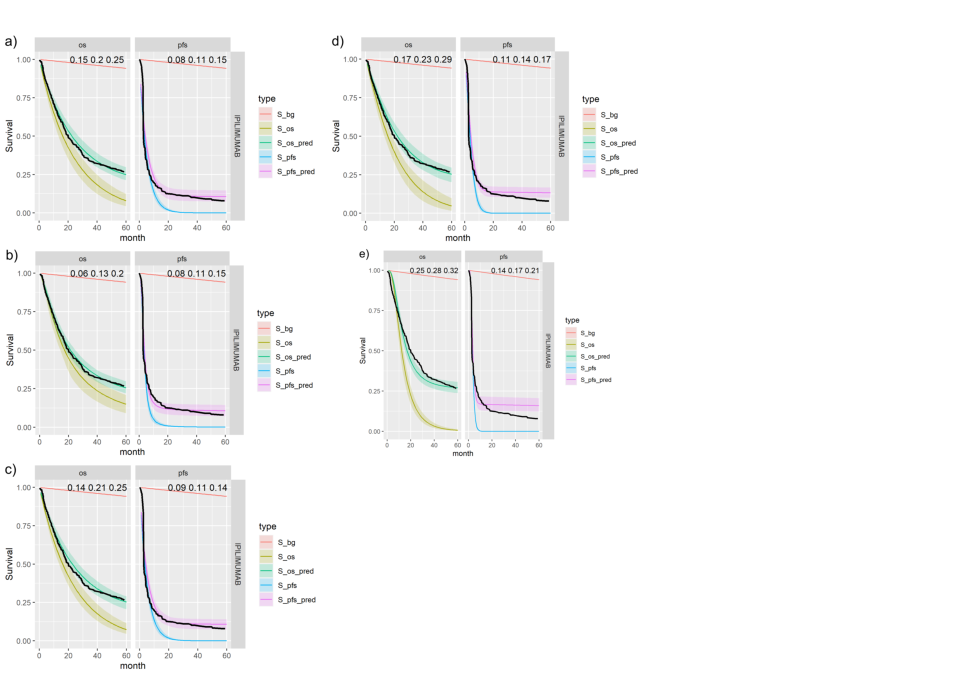
\includegraphics[width=25cm,height=40cm]{Check_mate_analysis_files/figure-latex/unnamed-chunk-8-1} 

}

\caption{\label{fig:IPI}Posterior survival curves for the mixture cure model with exchangeable cure fracion and $ipilimumab$. The red line is cured background, light green and blue are uncured, and dark green and magenta are combined. a) Exponential uncured b) Log-logistic uncured c) Gompertz uncured d) Weibull uncured e) Log-Normal uncured.}\label{fig:unnamed-chunk-8}
\end{figure}

\begin{figure}

{\centering 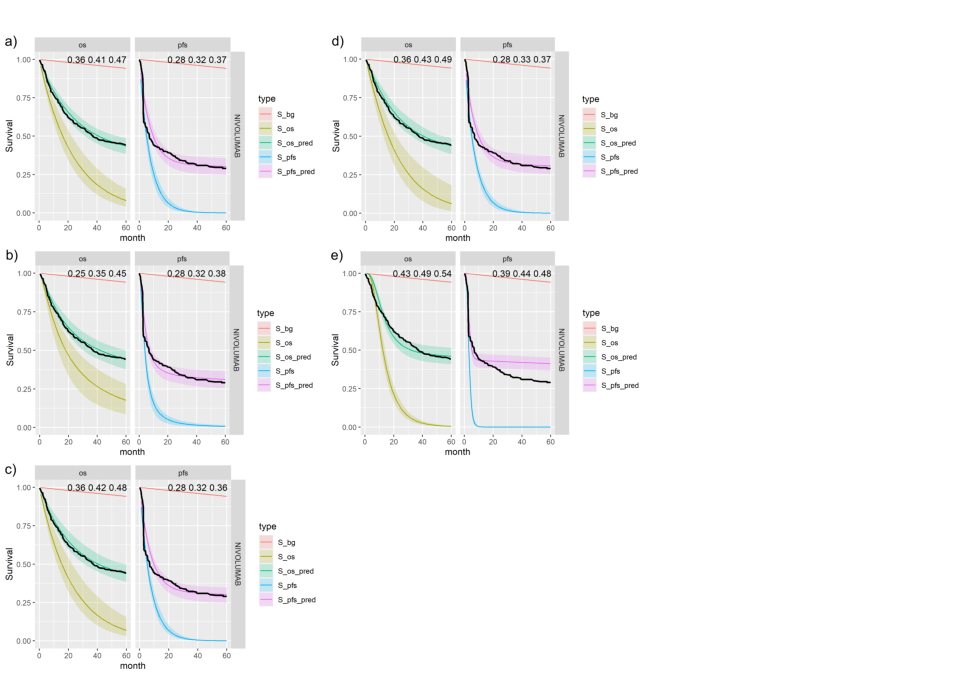
\includegraphics[width=25cm,height=40cm]{Check_mate_analysis_files/figure-latex/unnamed-chunk-9-1} 

}

\caption{\label{fig:NIVO}Posterior survival curves for the mixture cure model with exchangeable cure fracion and $nivolumab$. The red line is cured background, light green and blue are uncured, and dark green and magenta are combined. a) Exponential uncured b) Log-logistic uncured c) Gompertz uncured d) Weibull uncured e) Log-Normal uncured.}\label{fig:unnamed-chunk-9}
\end{figure}

\begin{figure}

{\centering 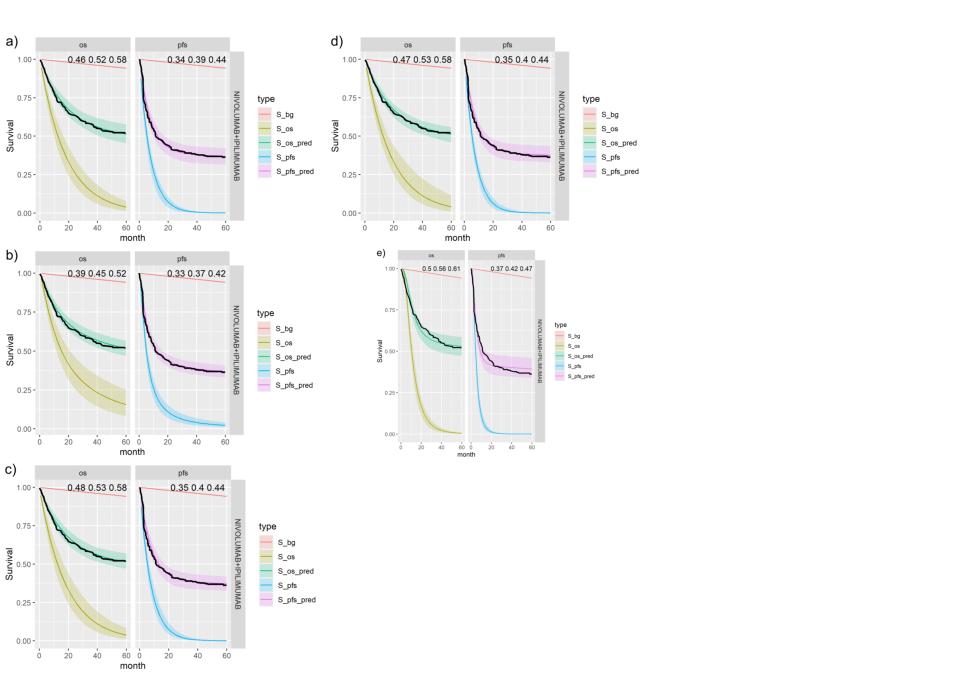
\includegraphics[width=25cm,height=40cm]{Check_mate_analysis_files/figure-latex/unnamed-chunk-10-1} 

}

\caption{\label{fig:NIVO+IPI}Posterior survival curves for the mixture cure model with exchangeable cure fracion and dual $ipilimumab$ and $nivolumab$. The red line is cured background, light green and blue are uncured, and dark green and magenta are combined. a) Exponential uncured b) Log-logistic uncured c) Gompertz uncured d) Weibull uncured e) Log-Normal uncured.}\label{fig:unnamed-chunk-10}
\end{figure}

Figures \ref{fig:forest_global}, \ref{fig:forest_os} and
\ref{fig:forest_pfs} show the forest plots of cure fraction posterior
distributions. We see that the values are generally similar for the
Exponential and log-logistic fits. This clearly shows how the global
cure fraction posterior distribution lies partway between the PFS and OS
distributions.

\begin{figure}

{\centering 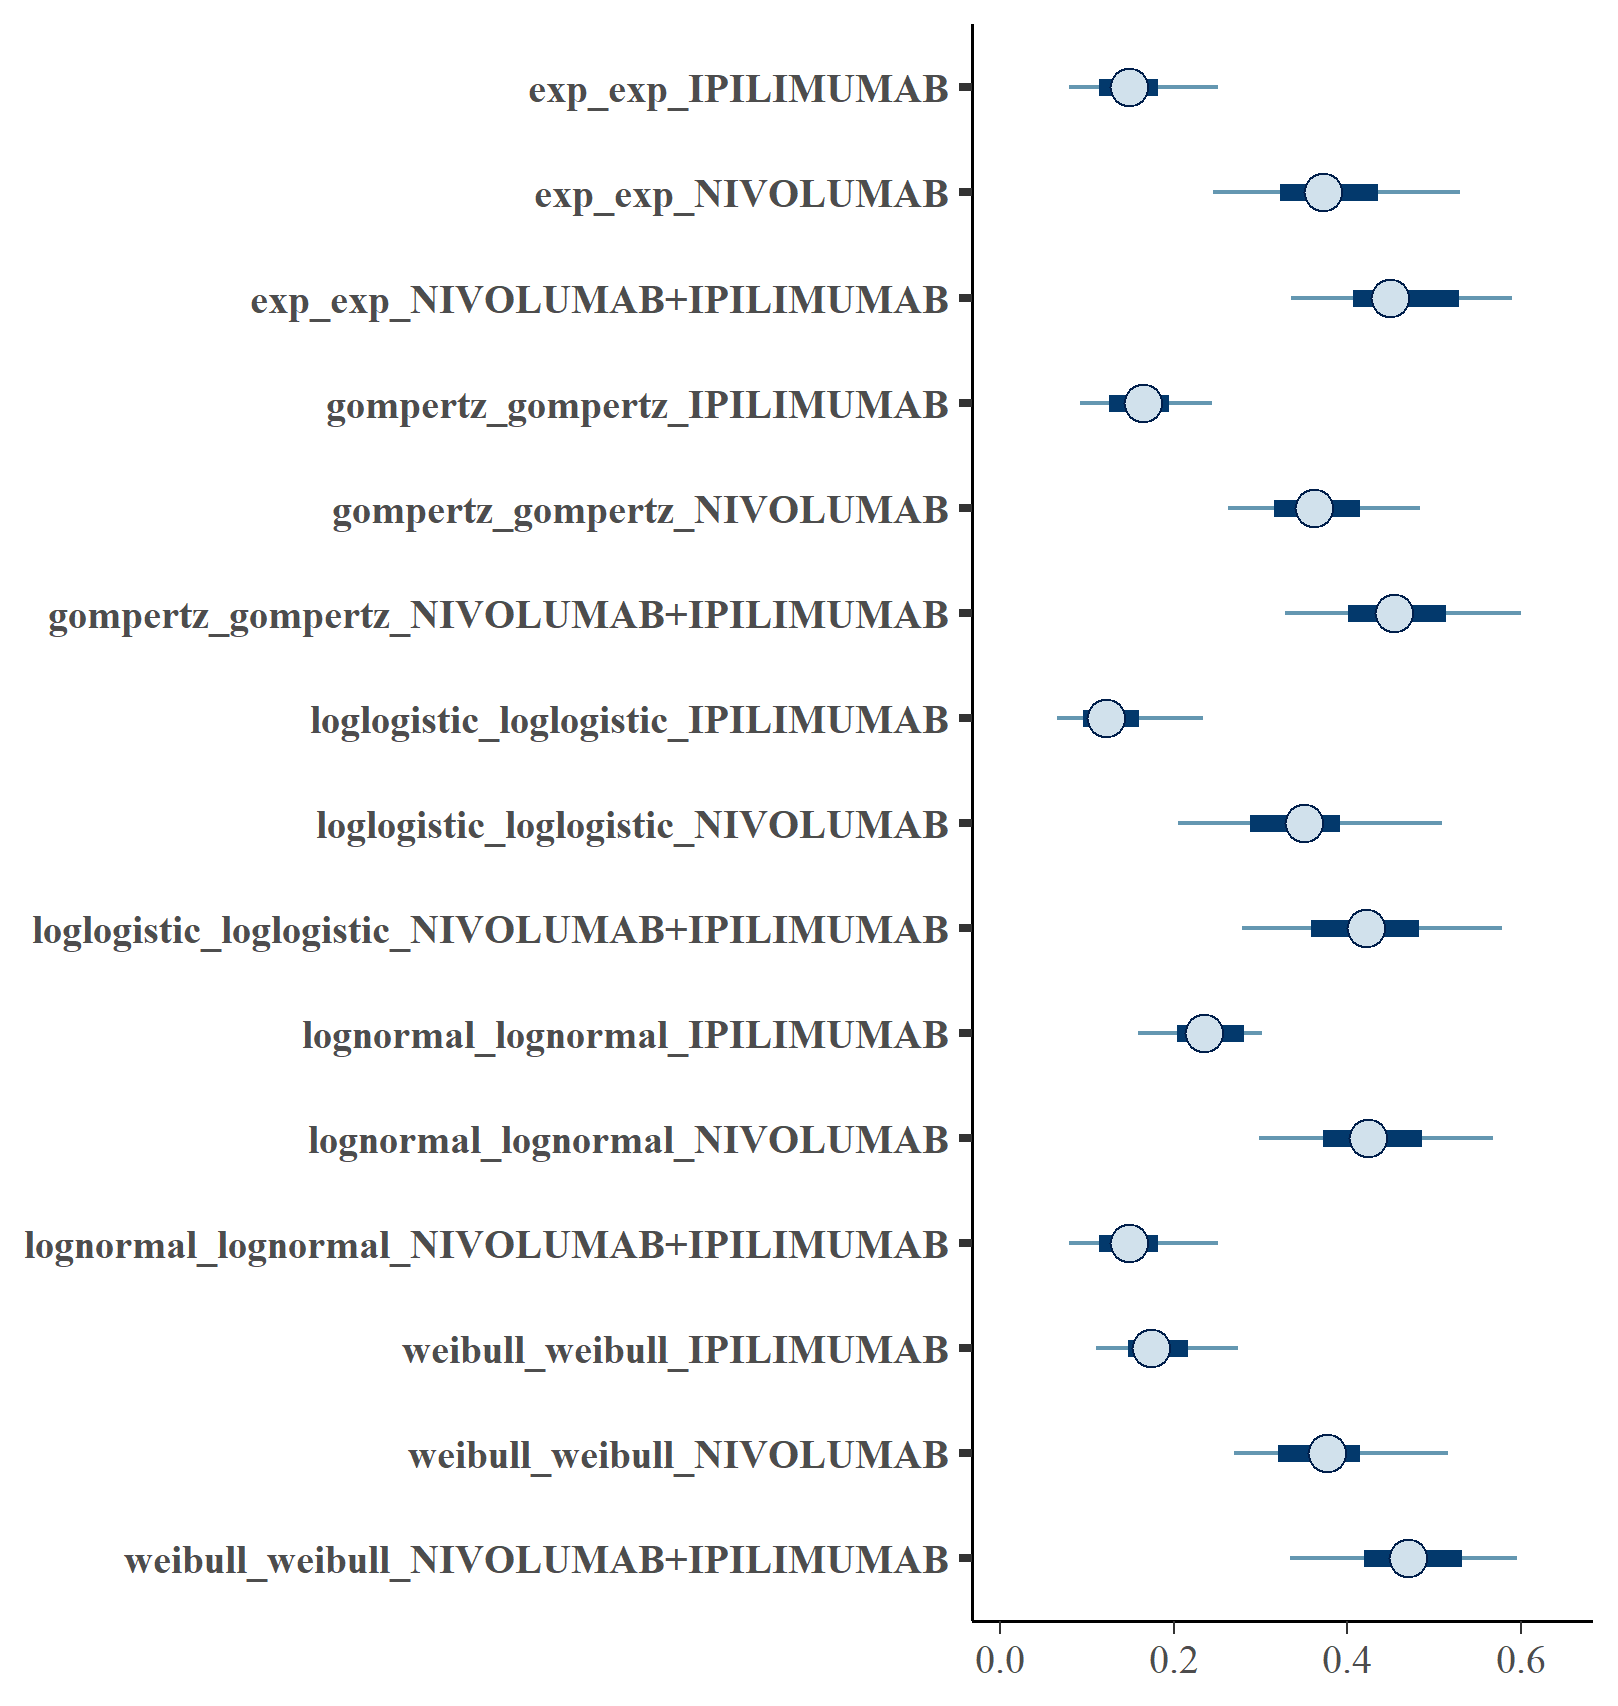
\includegraphics[width=0.6\linewidth]{../plots/cf_global_forest_plot} 

}

\caption{\label{fig:forest_global}Forest plot of global cure fraction posterior distributions.}\label{fig:unnamed-chunk-11}
\end{figure}

\begin{figure}

{\centering 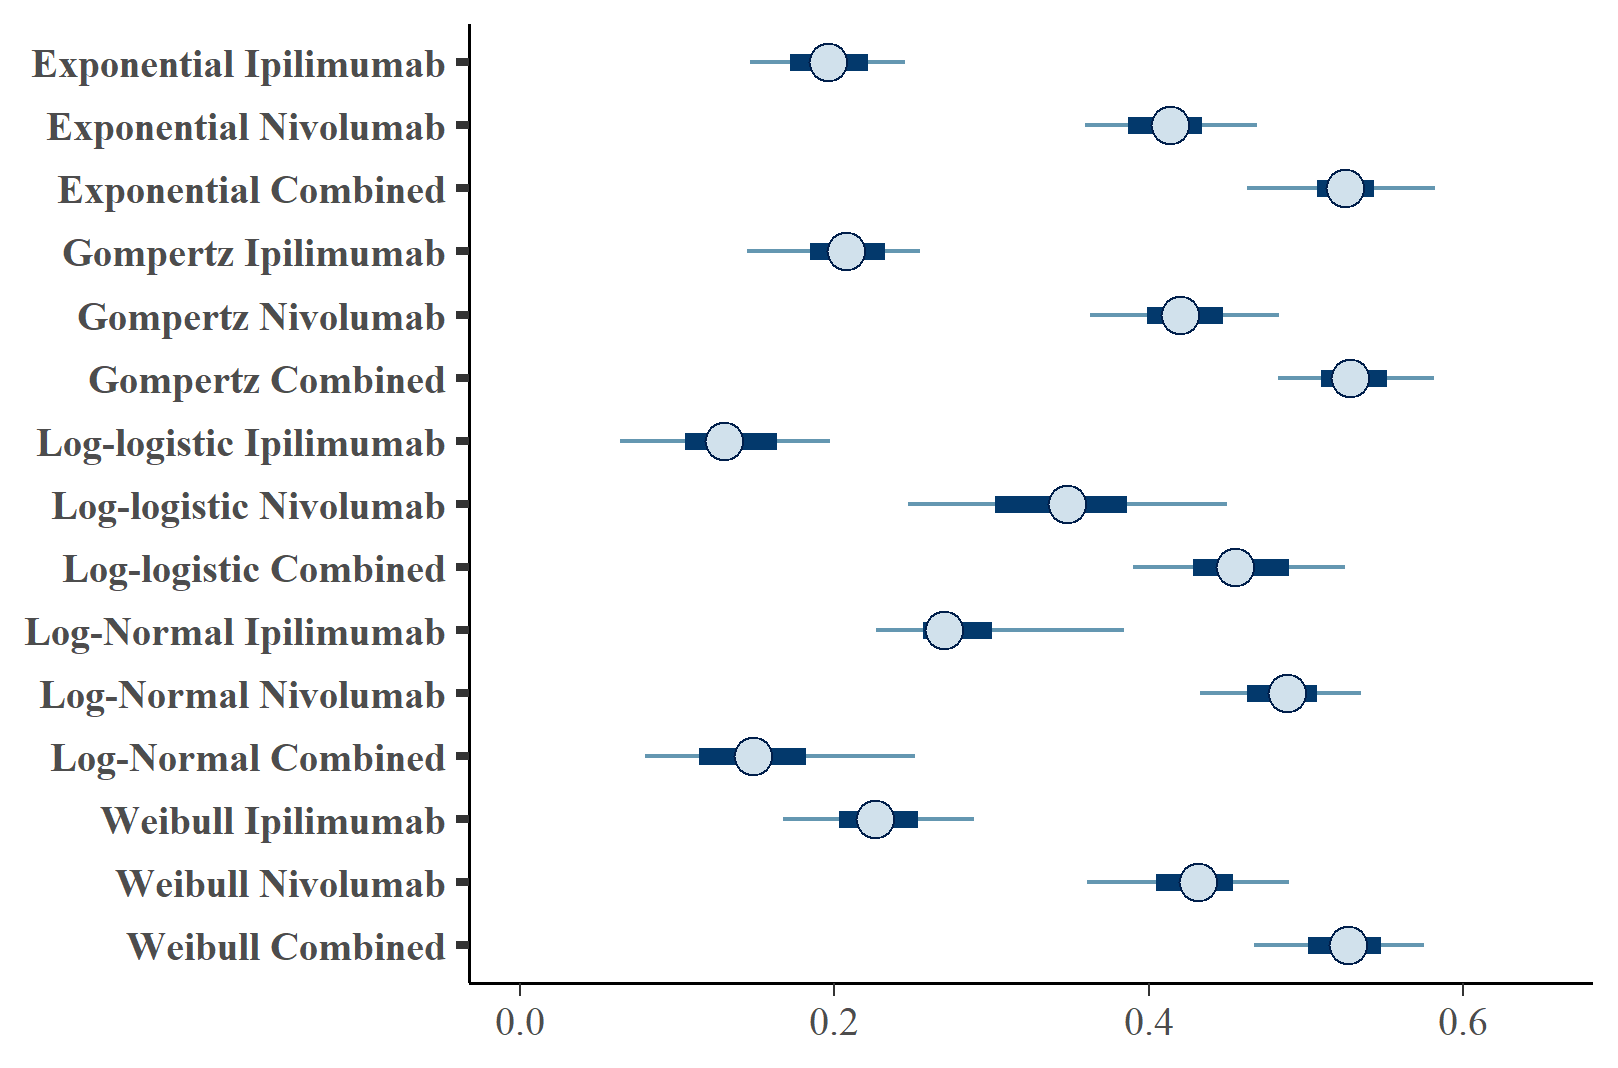
\includegraphics[width=0.6\linewidth]{../plots/cf_os_forest_plot} 

}

\caption{\label{fig:forest_os}Forest plot of OS cure fraction posterior distributions.}\label{fig:unnamed-chunk-12}
\end{figure}

\begin{figure}

{\centering 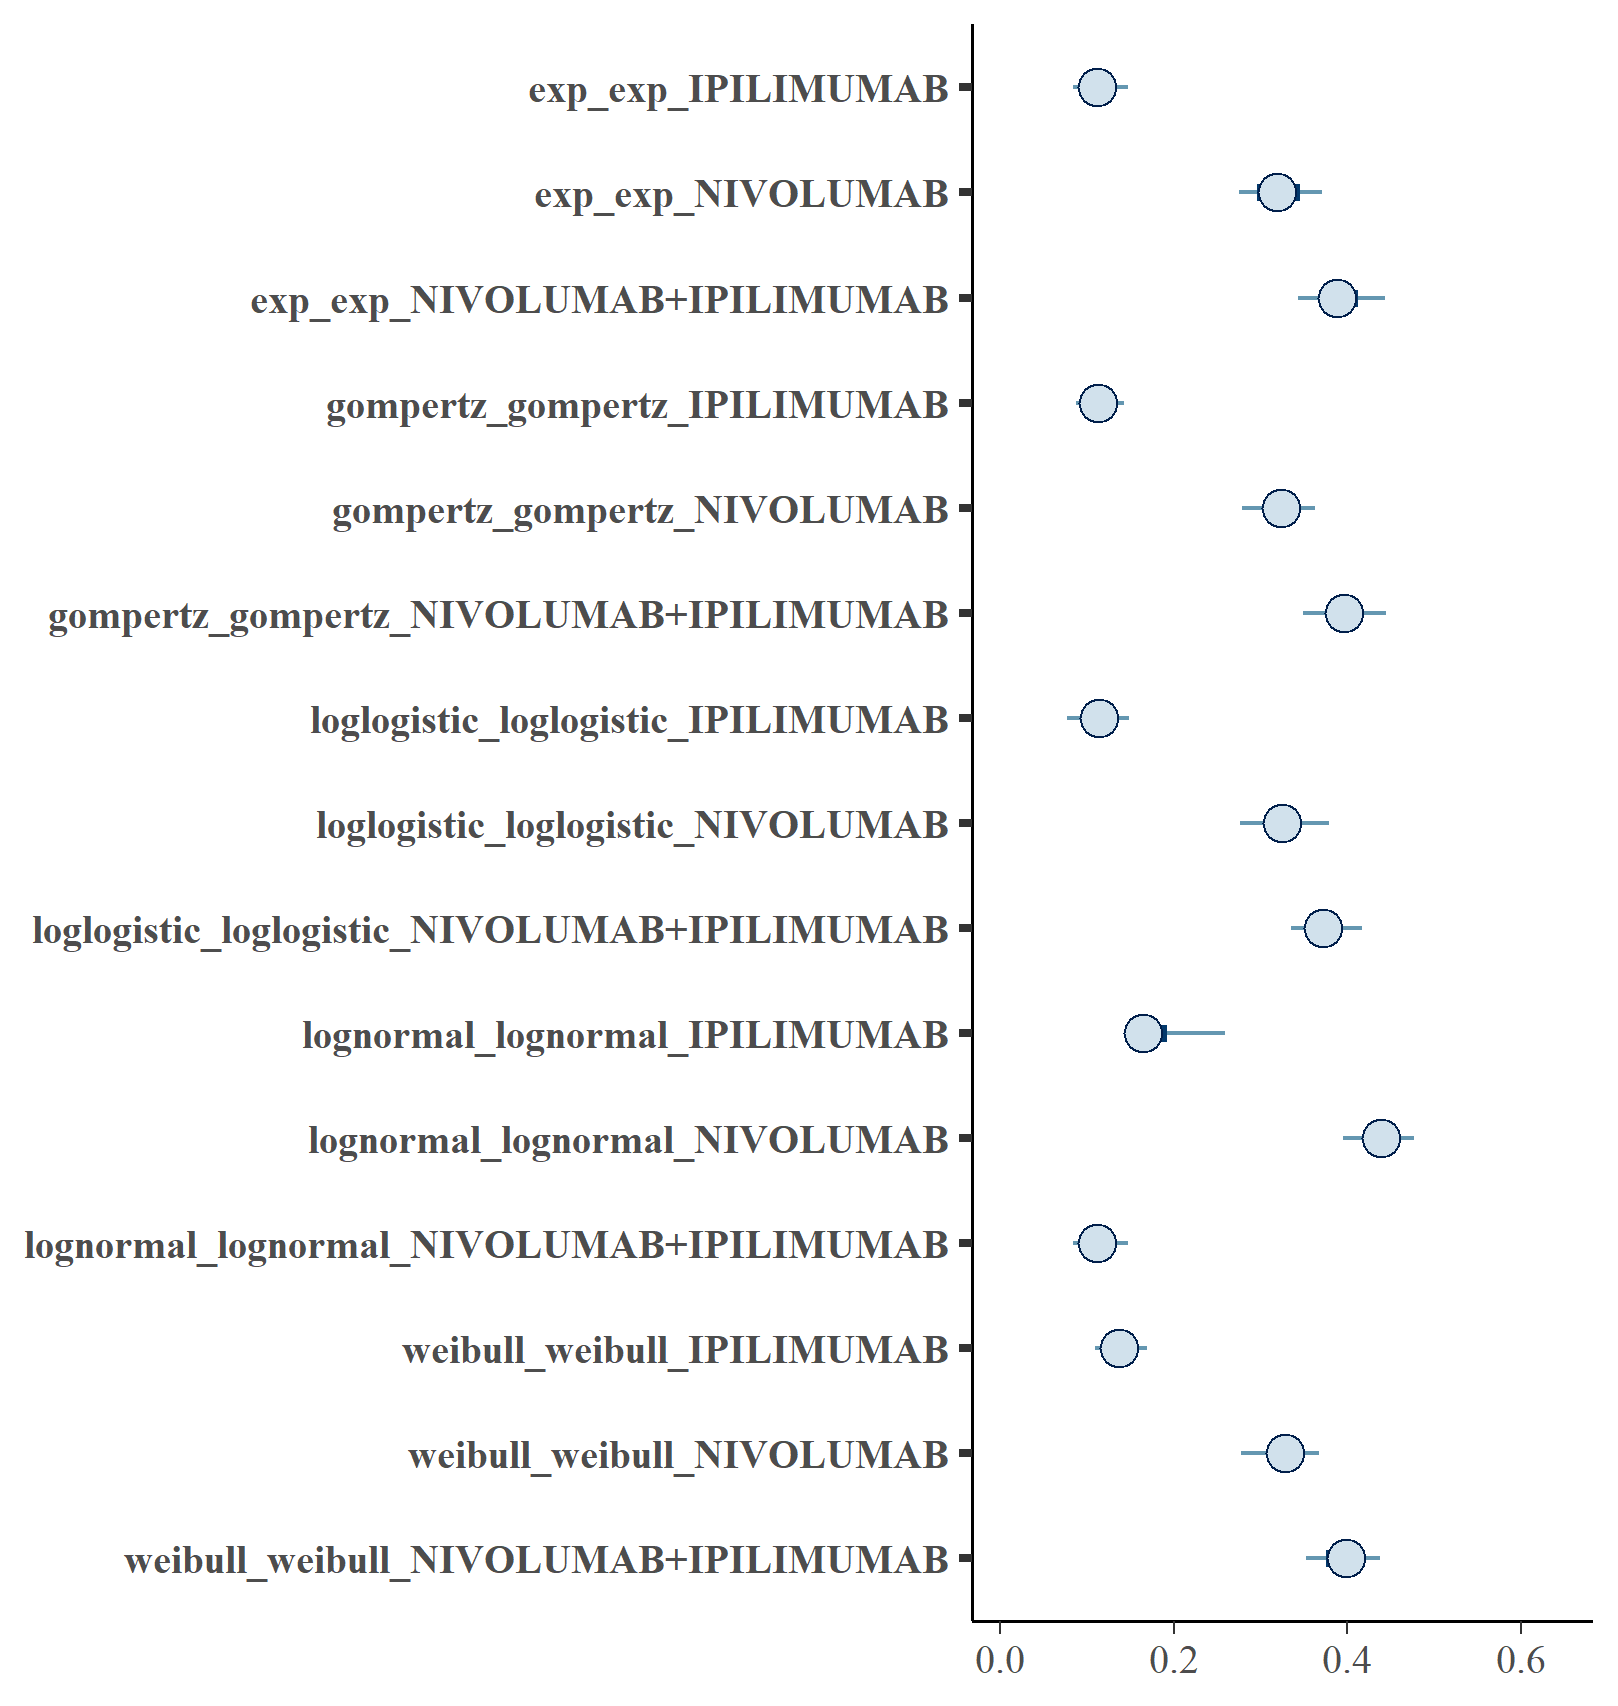
\includegraphics[width=0.6\linewidth]{../plots/cf_pfs_forest_plot} 

}

\caption{\label{fig:forest_pfs}Forest plot of PFS cure fraction posterior distributions.}\label{fig:unnamed-chunk-13}
\end{figure}

The table below summarises the cure fraction posterior distribution for
each scenario.

\begin{longtable}[]{@{}lllllll@{}}
\toprule
\begin{minipage}[b]{0.03\columnwidth}\raggedright
\strut
\end{minipage} & \begin{minipage}[b]{0.09\columnwidth}\raggedright
OS Distn\strut
\end{minipage} & \begin{minipage}[b]{0.09\columnwidth}\raggedright
PFS Distn\strut
\end{minipage} & \begin{minipage}[b]{0.15\columnwidth}\raggedright
Treatment\strut
\end{minipage} & \begin{minipage}[b]{0.15\columnwidth}\raggedright
\(cf\) (CrI)\strut
\end{minipage} & \begin{minipage}[b]{0.15\columnwidth}\raggedright
\(cf_{OS}\) (CrI)\strut
\end{minipage} & \begin{minipage}[b]{0.15\columnwidth}\raggedright
\(cf_{PFS}\) (CrI)\strut
\end{minipage}\tabularnewline
\midrule
\endhead
\begin{minipage}[t]{0.03\columnwidth}\raggedright
1\strut
\end{minipage} & \begin{minipage}[t]{0.09\columnwidth}\raggedright
exp\strut
\end{minipage} & \begin{minipage}[t]{0.09\columnwidth}\raggedright
exp\strut
\end{minipage} & \begin{minipage}[t]{0.15\columnwidth}\raggedright
IPILIMUMAB\strut
\end{minipage} & \begin{minipage}[t]{0.15\columnwidth}\raggedright
0.151 (0.068, 0.26)\strut
\end{minipage} & \begin{minipage}[t]{0.15\columnwidth}\raggedright
0.196 (0.136, 0.255)\strut
\end{minipage} & \begin{minipage}[t]{0.15\columnwidth}\raggedright
0.112 (0.079, 0.155)\strut
\end{minipage}\tabularnewline
\begin{minipage}[t]{0.03\columnwidth}\raggedright
2\strut
\end{minipage} & \begin{minipage}[t]{0.09\columnwidth}\raggedright
exp\strut
\end{minipage} & \begin{minipage}[t]{0.09\columnwidth}\raggedright
exp\strut
\end{minipage} & \begin{minipage}[t]{0.15\columnwidth}\raggedright
NIVOLUMAB\strut
\end{minipage} & \begin{minipage}[t]{0.15\columnwidth}\raggedright
0.378 (0.216, 0.557)\strut
\end{minipage} & \begin{minipage}[t]{0.15\columnwidth}\raggedright
0.412 (0.35, 0.479)\strut
\end{minipage} & \begin{minipage}[t]{0.15\columnwidth}\raggedright
0.321 (0.262, 0.379)\strut
\end{minipage}\tabularnewline
\begin{minipage}[t]{0.03\columnwidth}\raggedright
3\strut
\end{minipage} & \begin{minipage}[t]{0.09\columnwidth}\raggedright
exp\strut
\end{minipage} & \begin{minipage}[t]{0.09\columnwidth}\raggedright
exp\strut
\end{minipage} & \begin{minipage}[t]{0.15\columnwidth}\raggedright
NIVOLUMAB+IPILIMUMAB\strut
\end{minipage} & \begin{minipage}[t]{0.15\columnwidth}\raggedright
0.463 (0.328, 0.626)\strut
\end{minipage} & \begin{minipage}[t]{0.15\columnwidth}\raggedright
0.526 (0.452, 0.597)\strut
\end{minipage} & \begin{minipage}[t]{0.15\columnwidth}\raggedright
0.392 (0.334, 0.448)\strut
\end{minipage}\tabularnewline
\begin{minipage}[t]{0.03\columnwidth}\raggedright
4\strut
\end{minipage} & \begin{minipage}[t]{0.09\columnwidth}\raggedright
gompertz\strut
\end{minipage} & \begin{minipage}[t]{0.09\columnwidth}\raggedright
gompertz\strut
\end{minipage} & \begin{minipage}[t]{0.15\columnwidth}\raggedright
IPILIMUMAB\strut
\end{minipage} & \begin{minipage}[t]{0.15\columnwidth}\raggedright
0.164 (0.088, 0.275)\strut
\end{minipage} & \begin{minipage}[t]{0.15\columnwidth}\raggedright
0.207 (0.13, 0.266)\strut
\end{minipage} & \begin{minipage}[t]{0.15\columnwidth}\raggedright
0.114 (0.079, 0.148)\strut
\end{minipage}\tabularnewline
\begin{minipage}[t]{0.03\columnwidth}\raggedright
5\strut
\end{minipage} & \begin{minipage}[t]{0.09\columnwidth}\raggedright
gompertz\strut
\end{minipage} & \begin{minipage}[t]{0.09\columnwidth}\raggedright
gompertz\strut
\end{minipage} & \begin{minipage}[t]{0.15\columnwidth}\raggedright
NIVOLUMAB\strut
\end{minipage} & \begin{minipage}[t]{0.15\columnwidth}\raggedright
0.368 (0.247, 0.517)\strut
\end{minipage} & \begin{minipage}[t]{0.15\columnwidth}\raggedright
0.423 (0.358, 0.494)\strut
\end{minipage} & \begin{minipage}[t]{0.15\columnwidth}\raggedright
0.321 (0.261, 0.369)\strut
\end{minipage}\tabularnewline
\begin{minipage}[t]{0.03\columnwidth}\raggedright
6\strut
\end{minipage} & \begin{minipage}[t]{0.09\columnwidth}\raggedright
gompertz\strut
\end{minipage} & \begin{minipage}[t]{0.09\columnwidth}\raggedright
gompertz\strut
\end{minipage} & \begin{minipage}[t]{0.15\columnwidth}\raggedright
NIVOLUMAB+IPILIMUMAB\strut
\end{minipage} & \begin{minipage}[t]{0.15\columnwidth}\raggedright
0.458 (0.318, 0.612)\strut
\end{minipage} & \begin{minipage}[t]{0.15\columnwidth}\raggedright
0.529 (0.477, 0.594)\strut
\end{minipage} & \begin{minipage}[t]{0.15\columnwidth}\raggedright
0.395 (0.346, 0.446)\strut
\end{minipage}\tabularnewline
\begin{minipage}[t]{0.03\columnwidth}\raggedright
7\strut
\end{minipage} & \begin{minipage}[t]{0.09\columnwidth}\raggedright
loglogistic\strut
\end{minipage} & \begin{minipage}[t]{0.09\columnwidth}\raggedright
loglogistic\strut
\end{minipage} & \begin{minipage}[t]{0.15\columnwidth}\raggedright
IPILIMUMAB\strut
\end{minipage} & \begin{minipage}[t]{0.15\columnwidth}\raggedright
0.133 (0.061, 0.278)\strut
\end{minipage} & \begin{minipage}[t]{0.15\columnwidth}\raggedright
0.133 (0.054, 0.206)\strut
\end{minipage} & \begin{minipage}[t]{0.15\columnwidth}\raggedright
0.113 (0.075, 0.152)\strut
\end{minipage}\tabularnewline
\begin{minipage}[t]{0.03\columnwidth}\raggedright
8\strut
\end{minipage} & \begin{minipage}[t]{0.09\columnwidth}\raggedright
loglogistic\strut
\end{minipage} & \begin{minipage}[t]{0.09\columnwidth}\raggedright
loglogistic\strut
\end{minipage} & \begin{minipage}[t]{0.15\columnwidth}\raggedright
NIVOLUMAB\strut
\end{minipage} & \begin{minipage}[t]{0.15\columnwidth}\raggedright
0.348 (0.191, 0.526)\strut
\end{minipage} & \begin{minipage}[t]{0.15\columnwidth}\raggedright
0.345 (0.231, 0.456)\strut
\end{minipage} & \begin{minipage}[t]{0.15\columnwidth}\raggedright
0.325 (0.264, 0.382)\strut
\end{minipage}\tabularnewline
\begin{minipage}[t]{0.03\columnwidth}\raggedright
9\strut
\end{minipage} & \begin{minipage}[t]{0.09\columnwidth}\raggedright
loglogistic\strut
\end{minipage} & \begin{minipage}[t]{0.09\columnwidth}\raggedright
loglogistic\strut
\end{minipage} & \begin{minipage}[t]{0.15\columnwidth}\raggedright
NIVOLUMAB+IPILIMUMAB\strut
\end{minipage} & \begin{minipage}[t]{0.15\columnwidth}\raggedright
0.421 (0.266, 0.599)\strut
\end{minipage} & \begin{minipage}[t]{0.15\columnwidth}\raggedright
0.459 (0.37, 0.535)\strut
\end{minipage} & \begin{minipage}[t]{0.15\columnwidth}\raggedright
0.375 (0.327, 0.421)\strut
\end{minipage}\tabularnewline
\begin{minipage}[t]{0.03\columnwidth}\raggedright
10\strut
\end{minipage} & \begin{minipage}[t]{0.09\columnwidth}\raggedright
lognormal\strut
\end{minipage} & \begin{minipage}[t]{0.09\columnwidth}\raggedright
lognormal\strut
\end{minipage} & \begin{minipage}[t]{0.15\columnwidth}\raggedright
IPILIMUMAB\strut
\end{minipage} & \begin{minipage}[t]{0.15\columnwidth}\raggedright
0.236 (0.127, 0.303)\strut
\end{minipage} & \begin{minipage}[t]{0.15\columnwidth}\raggedright
0.285 (0.198, 0.468)\strut
\end{minipage} & \begin{minipage}[t]{0.15\columnwidth}\raggedright
0.177 (0.136, 0.293)\strut
\end{minipage}\tabularnewline
\begin{minipage}[t]{0.03\columnwidth}\raggedright
11\strut
\end{minipage} & \begin{minipage}[t]{0.09\columnwidth}\raggedright
lognormal\strut
\end{minipage} & \begin{minipage}[t]{0.09\columnwidth}\raggedright
lognormal\strut
\end{minipage} & \begin{minipage}[t]{0.15\columnwidth}\raggedright
NIVOLUMAB\strut
\end{minipage} & \begin{minipage}[t]{0.15\columnwidth}\raggedright
0.425 (0.286, 0.588)\strut
\end{minipage} & \begin{minipage}[t]{0.15\columnwidth}\raggedright
0.486 (0.431, 0.546)\strut
\end{minipage} & \begin{minipage}[t]{0.15\columnwidth}\raggedright
0.437 (0.39, 0.48)\strut
\end{minipage}\tabularnewline
\begin{minipage}[t]{0.03\columnwidth}\raggedright
12\strut
\end{minipage} & \begin{minipage}[t]{0.09\columnwidth}\raggedright
lognormal\strut
\end{minipage} & \begin{minipage}[t]{0.09\columnwidth}\raggedright
lognormal\strut
\end{minipage} & \begin{minipage}[t]{0.15\columnwidth}\raggedright
NIVOLUMAB+IPILIMUMAB\strut
\end{minipage} & \begin{minipage}[t]{0.15\columnwidth}\raggedright
0.431 (0.301, 0.581)\strut
\end{minipage} & \begin{minipage}[t]{0.15\columnwidth}\raggedright
0.556 (0.494, 0.619)\strut
\end{minipage} & \begin{minipage}[t]{0.15\columnwidth}\raggedright
0.42 (0.37, 0.481)\strut
\end{minipage}\tabularnewline
\begin{minipage}[t]{0.03\columnwidth}\raggedright
13\strut
\end{minipage} & \begin{minipage}[t]{0.09\columnwidth}\raggedright
weibull\strut
\end{minipage} & \begin{minipage}[t]{0.09\columnwidth}\raggedright
weibull\strut
\end{minipage} & \begin{minipage}[t]{0.15\columnwidth}\raggedright
IPILIMUMAB\strut
\end{minipage} & \begin{minipage}[t]{0.15\columnwidth}\raggedright
0.184 (0.095, 0.29)\strut
\end{minipage} & \begin{minipage}[t]{0.15\columnwidth}\raggedright
0.229 (0.157, 0.295)\strut
\end{minipage} & \begin{minipage}[t]{0.15\columnwidth}\raggedright
0.141 (0.107, 0.177)\strut
\end{minipage}\tabularnewline
\begin{minipage}[t]{0.03\columnwidth}\raggedright
14\strut
\end{minipage} & \begin{minipage}[t]{0.09\columnwidth}\raggedright
weibull\strut
\end{minipage} & \begin{minipage}[t]{0.09\columnwidth}\raggedright
weibull\strut
\end{minipage} & \begin{minipage}[t]{0.15\columnwidth}\raggedright
NIVOLUMAB\strut
\end{minipage} & \begin{minipage}[t]{0.15\columnwidth}\raggedright
0.375 (0.242, 0.541)\strut
\end{minipage} & \begin{minipage}[t]{0.15\columnwidth}\raggedright
0.427 (0.346, 0.494)\strut
\end{minipage} & \begin{minipage}[t]{0.15\columnwidth}\raggedright
0.326 (0.27, 0.394)\strut
\end{minipage}\tabularnewline
\begin{minipage}[t]{0.03\columnwidth}\raggedright
15\strut
\end{minipage} & \begin{minipage}[t]{0.09\columnwidth}\raggedright
weibull\strut
\end{minipage} & \begin{minipage}[t]{0.09\columnwidth}\raggedright
weibull\strut
\end{minipage} & \begin{minipage}[t]{0.15\columnwidth}\raggedright
NIVOLUMAB+IPILIMUMAB\strut
\end{minipage} & \begin{minipage}[t]{0.15\columnwidth}\raggedright
0.471 (0.328, 0.647)\strut
\end{minipage} & \begin{minipage}[t]{0.15\columnwidth}\raggedright
0.523 (0.461, 0.58)\strut
\end{minipage} & \begin{minipage}[t]{0.15\columnwidth}\raggedright
0.399 (0.35, 0.462)\strut
\end{minipage}\tabularnewline
\bottomrule
\end{longtable}

The table below gives the leave-one-out cross validation statistics for
each model fit.

\begin{longtable}[]{@{}llllrr@{}}
\toprule
OS Distn & PFS Distn & Treatment & Statistic & Estimate &
SE\tabularnewline
\midrule
\endhead
exp & exp & IPILIMUMAB & elpd\_waic & -1838.83 & 36.07\tabularnewline
exp & exp & NIVOLUMAB & elpd\_waic & -1679.59 & 45.69\tabularnewline
exp & exp & NIVOLUMAB+IPILIMUMAB & elpd\_waic & -1549.68 &
60.15\tabularnewline
gompertz & gompertz & IPILIMUMAB & elpd\_waic & -1488.81 &
58.20\tabularnewline
gompertz & gompertz & NIVOLUMAB & elpd\_waic & -1819.89 &
39.69\tabularnewline
gompertz & gompertz & NIVOLUMAB+IPILIMUMAB & elpd\_waic & -1680.25 &
45.91\tabularnewline
loglogistic & loglogistic & IPILIMUMAB & elpd\_waic & -1544.04 &
54.19\tabularnewline
loglogistic & loglogistic & NIVOLUMAB & elpd\_waic & -1543.49 &
53.87\tabularnewline
loglogistic & loglogistic & NIVOLUMAB+IPILIMUMAB & elpd\_waic & -1839.34
& 36.27\tabularnewline
lognormal & lognormal & IPILIMUMAB & elpd\_waic & -1679.48 &
45.80\tabularnewline
lognormal & lognormal & NIVOLUMAB & elpd\_waic & -1543.81 &
54.03\tabularnewline
lognormal & lognormal & NIVOLUMAB+IPILIMUMAB & elpd\_waic & -1768.17 &
39.20\tabularnewline
weibull & weibull & IPILIMUMAB & elpd\_waic & -1651.73 &
46.02\tabularnewline
weibull & weibull & NIVOLUMAB & elpd\_waic & -1533.95 &
53.17\tabularnewline
weibull & weibull & NIVOLUMAB+IPILIMUMAB & elpd\_waic & -1566.33 &
55.91\tabularnewline
exp & exp & IPILIMUMAB & p\_waic & 5.37 & 0.48\tabularnewline
exp & exp & NIVOLUMAB & p\_waic & 7.45 & 0.62\tabularnewline
exp & exp & NIVOLUMAB+IPILIMUMAB & p\_waic & 15.46 & 1.44\tabularnewline
gompertz & gompertz & IPILIMUMAB & p\_waic & 14.55 & 1.26\tabularnewline
gompertz & gompertz & NIVOLUMAB & p\_waic & 9.46 & 0.96\tabularnewline
gompertz & gompertz & NIVOLUMAB+IPILIMUMAB & p\_waic & 8.70 &
0.75\tabularnewline
loglogistic & loglogistic & IPILIMUMAB & p\_waic & 7.70 &
0.72\tabularnewline
loglogistic & loglogistic & NIVOLUMAB & p\_waic & 7.15 &
0.60\tabularnewline
loglogistic & loglogistic & NIVOLUMAB+IPILIMUMAB & p\_waic & 5.91 &
0.52\tabularnewline
lognormal & lognormal & IPILIMUMAB & p\_waic & 6.96 &
0.56\tabularnewline
lognormal & lognormal & NIVOLUMAB & p\_waic & 7.07 & 0.78\tabularnewline
lognormal & lognormal & NIVOLUMAB+IPILIMUMAB & p\_waic & 9.19 &
0.56\tabularnewline
weibull & weibull & IPILIMUMAB & p\_waic & 9.20 & 0.53\tabularnewline
weibull & weibull & NIVOLUMAB & p\_waic & 6.10 & 0.50\tabularnewline
weibull & weibull & NIVOLUMAB+IPILIMUMAB & p\_waic & 20.04 &
1.20\tabularnewline
exp & exp & IPILIMUMAB & waic & 3677.65 & 72.13\tabularnewline
exp & exp & NIVOLUMAB & waic & 3359.19 & 91.37\tabularnewline
exp & exp & NIVOLUMAB+IPILIMUMAB & waic & 3099.36 &
120.30\tabularnewline
gompertz & gompertz & IPILIMUMAB & waic & 2977.62 &
116.41\tabularnewline
gompertz & gompertz & NIVOLUMAB & waic & 3639.77 & 79.38\tabularnewline
gompertz & gompertz & NIVOLUMAB+IPILIMUMAB & waic & 3360.49 &
91.83\tabularnewline
loglogistic & loglogistic & IPILIMUMAB & waic & 3088.08 &
108.39\tabularnewline
loglogistic & loglogistic & NIVOLUMAB & waic & 3086.98 &
107.74\tabularnewline
loglogistic & loglogistic & NIVOLUMAB+IPILIMUMAB & waic & 3678.68 &
72.53\tabularnewline
lognormal & lognormal & IPILIMUMAB & waic & 3358.96 &
91.59\tabularnewline
lognormal & lognormal & NIVOLUMAB & waic & 3087.62 &
108.05\tabularnewline
lognormal & lognormal & NIVOLUMAB+IPILIMUMAB & waic & 3536.33 &
78.40\tabularnewline
weibull & weibull & IPILIMUMAB & waic & 3303.47 & 92.04\tabularnewline
weibull & weibull & NIVOLUMAB & waic & 3067.91 & 106.35\tabularnewline
weibull & weibull & NIVOLUMAB+IPILIMUMAB & waic & 3132.66 &
111.82\tabularnewline
\bottomrule
\end{longtable}

The variance partition coefficient (VPC) is defined as
\(\sigma_{global}^2/ (\sigma_{global}^2 + \sigma_{e}^2)\) where
\(e = PFS\) or \(OS\). This indicates want proportion of the total
variance is attributable to variation within-groups, or how much is
found between-groups.

\begin{longtable}[]{@{}lllrr@{}}
\toprule
OS Distn & PFS Distn & Treatment & PFS & OS\tabularnewline
\midrule
\endhead
exp & exp & IPILIMUMAB & 0.813 & 0.784\tabularnewline
exp & exp & NIVOLUMAB & 0.876 & 0.877\tabularnewline
exp & exp & NIVOLUMAB+IPILIMUMAB & 0.865 & 0.860\tabularnewline
gompertz & gompertz & IPILIMUMAB & 0.781 & 0.743\tabularnewline
gompertz & gompertz & NIVOLUMAB & 0.858 & 0.808\tabularnewline
gompertz & gompertz & NIVOLUMAB+IPILIMUMAB & 0.899 &
0.888\tabularnewline
loglogistic & loglogistic & IPILIMUMAB & 0.812 & 0.604\tabularnewline
loglogistic & loglogistic & NIVOLUMAB & 0.890 & 0.672\tabularnewline
loglogistic & loglogistic & NIVOLUMAB+IPILIMUMAB & 0.915 &
0.786\tabularnewline
lognormal & lognormal & IPILIMUMAB & 0.607 & 0.513\tabularnewline
lognormal & lognormal & NIVOLUMAB & 0.928 & 0.881\tabularnewline
lognormal & lognormal & NIVOLUMAB+IPILIMUMAB & 0.868 &
0.862\tabularnewline
weibull & weibull & IPILIMUMAB & 0.841 & 0.726\tabularnewline
weibull & weibull & NIVOLUMAB & 0.865 & 0.822\tabularnewline
weibull & weibull & NIVOLUMAB+IPILIMUMAB & 0.891 & 0.863\tabularnewline
\bottomrule
\end{longtable}

It appears the above table that much of the variation is due to between
PFS and OS indicating distinct cure fractions in each.

\hypertarget{sensitivity-analysis-for-background-mortality}{%
\subsection{Sensitivity analysis for background
mortality}\label{sensitivity-analysis-for-background-mortality}}

As a sensitivity analysis, an adjustment factor was applied to the
general population mortality rates to allow for an assessment of the
impact of background hazards on estimation of the cure fraction. A
hazard ratio of 1.63 was applied to the background hazard. This was
obtained from a previous ad-hoc analysis which compared the WHO life
tables with the OS data for complete responders (CR) from CheckMate 067
(N=120, pooled across all 3 arms).

Figure \ref{fig:NIVO+IPI_163} shows the equivalent posterior survival
curves to Figure \ref{fig:NIVO+IPI} for the combined \(ipilimumab\) and
\(nivolumab\) treatment and background hazard ratio adjustment 1.63.
There is a small increase of approximately 1-2\% in the cure fraction
estimates.

\begin{figure}

{\centering 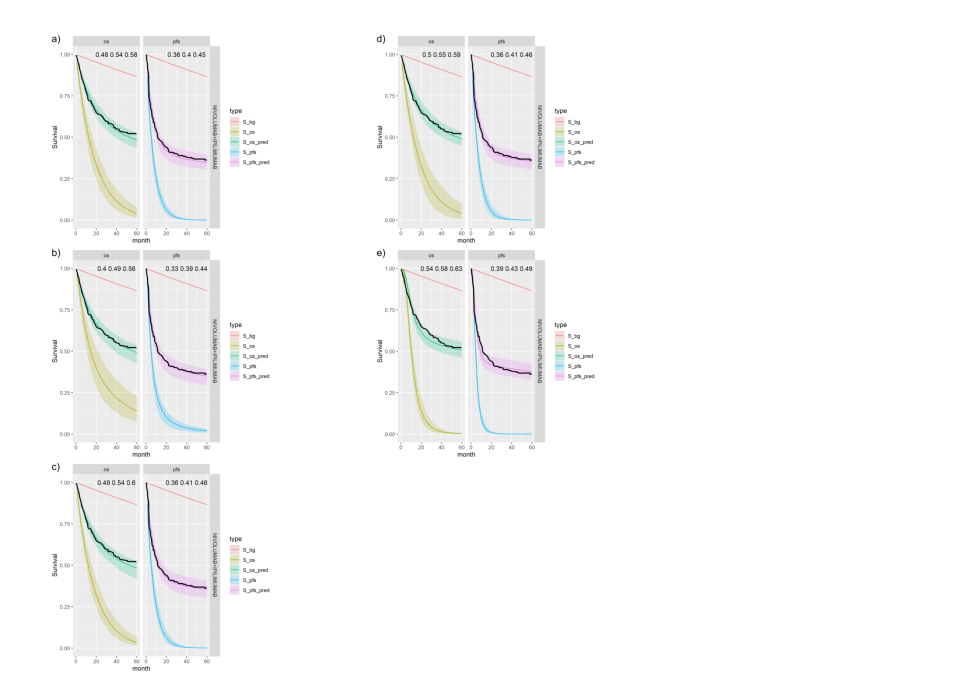
\includegraphics[width=25cm,height=40cm]{Check_mate_analysis_files/figure-latex/unnamed-chunk-14-1} 

}

\caption{\label{fig:NIVO+IPI_163}Posterior survival curves for the mixture cure model with exchangeable cure fracion and dual $ipilimumab$ and $nivolumab$ and background hazard ratio adjustment 1.63. The red line is cured background, light green and blue are uncured, and dark green and magenta are combined. a) Exponential uncured b) Log-logistic uncured c) Gompertz uncured d) Weibull uncured e) Log-Normal uncured.}\label{fig:unnamed-chunk-14}
\end{figure}

The table below summarises the cure fraction posterior distribution for
each scenario.

\begin{longtable}[]{@{}lllllll@{}}
\toprule
\begin{minipage}[b]{0.02\columnwidth}\raggedright
\strut
\end{minipage} & \begin{minipage}[b]{0.09\columnwidth}\raggedright
OS Distn\strut
\end{minipage} & \begin{minipage}[b]{0.09\columnwidth}\raggedright
PFS Distn\strut
\end{minipage} & \begin{minipage}[b]{0.15\columnwidth}\raggedright
Treatment\strut
\end{minipage} & \begin{minipage}[b]{0.15\columnwidth}\raggedright
\(cf\) (CrI)\strut
\end{minipage} & \begin{minipage}[b]{0.15\columnwidth}\raggedright
\(cf_{OS}\) (CrI)\strut
\end{minipage} & \begin{minipage}[b]{0.15\columnwidth}\raggedright
\(cf_{PFS}\) (CrI)\strut
\end{minipage}\tabularnewline
\midrule
\endhead
\begin{minipage}[t]{0.02\columnwidth}\raggedright
1\strut
\end{minipage} & \begin{minipage}[t]{0.09\columnwidth}\raggedright
exp\strut
\end{minipage} & \begin{minipage}[t]{0.09\columnwidth}\raggedright
exp\strut
\end{minipage} & \begin{minipage}[t]{0.15\columnwidth}\raggedright
NIVOLUMAB+IPILIMUMAB\strut
\end{minipage} & \begin{minipage}[t]{0.15\columnwidth}\raggedright
0.45 (0.291, 0.646)\strut
\end{minipage} & \begin{minipage}[t]{0.15\columnwidth}\raggedright
0.538 (0.473, 0.588)\strut
\end{minipage} & \begin{minipage}[t]{0.15\columnwidth}\raggedright
0.402 (0.351, 0.457)\strut
\end{minipage}\tabularnewline
\begin{minipage}[t]{0.02\columnwidth}\raggedright
2\strut
\end{minipage} & \begin{minipage}[t]{0.09\columnwidth}\raggedright
gompertz\strut
\end{minipage} & \begin{minipage}[t]{0.09\columnwidth}\raggedright
gompertz\strut
\end{minipage} & \begin{minipage}[t]{0.15\columnwidth}\raggedright
NIVOLUMAB+IPILIMUMAB\strut
\end{minipage} & \begin{minipage}[t]{0.15\columnwidth}\raggedright
0.459 (0.287, 0.616)\strut
\end{minipage} & \begin{minipage}[t]{0.15\columnwidth}\raggedright
0.541 (0.448, 0.6)\strut
\end{minipage} & \begin{minipage}[t]{0.15\columnwidth}\raggedright
0.409 (0.349, 0.474)\strut
\end{minipage}\tabularnewline
\begin{minipage}[t]{0.02\columnwidth}\raggedright
3\strut
\end{minipage} & \begin{minipage}[t]{0.09\columnwidth}\raggedright
loglogistic\strut
\end{minipage} & \begin{minipage}[t]{0.09\columnwidth}\raggedright
loglogistic\strut
\end{minipage} & \begin{minipage}[t]{0.15\columnwidth}\raggedright
NIVOLUMAB+IPILIMUMAB\strut
\end{minipage} & \begin{minipage}[t]{0.15\columnwidth}\raggedright
0.433 (0.287, 0.601)\strut
\end{minipage} & \begin{minipage}[t]{0.15\columnwidth}\raggedright
0.482 (0.374, 0.567)\strut
\end{minipage} & \begin{minipage}[t]{0.15\columnwidth}\raggedright
0.39 (0.324, 0.444)\strut
\end{minipage}\tabularnewline
\begin{minipage}[t]{0.02\columnwidth}\raggedright
4\strut
\end{minipage} & \begin{minipage}[t]{0.09\columnwidth}\raggedright
lognormal\strut
\end{minipage} & \begin{minipage}[t]{0.09\columnwidth}\raggedright
lognormal\strut
\end{minipage} & \begin{minipage}[t]{0.15\columnwidth}\raggedright
NIVOLUMAB+IPILIMUMAB\strut
\end{minipage} & \begin{minipage}[t]{0.15\columnwidth}\raggedright
0.46 (0.289, 0.648)\strut
\end{minipage} & \begin{minipage}[t]{0.15\columnwidth}\raggedright
0.583 (0.531, 0.643)\strut
\end{minipage} & \begin{minipage}[t]{0.15\columnwidth}\raggedright
0.434 (0.381, 0.491)\strut
\end{minipage}\tabularnewline
\begin{minipage}[t]{0.02\columnwidth}\raggedright
5\strut
\end{minipage} & \begin{minipage}[t]{0.09\columnwidth}\raggedright
weibull\strut
\end{minipage} & \begin{minipage}[t]{0.09\columnwidth}\raggedright
weibull\strut
\end{minipage} & \begin{minipage}[t]{0.15\columnwidth}\raggedright
NIVOLUMAB+IPILIMUMAB\strut
\end{minipage} & \begin{minipage}[t]{0.15\columnwidth}\raggedright
0.469 (0.297, 0.62)\strut
\end{minipage} & \begin{minipage}[t]{0.15\columnwidth}\raggedright
0.546 (0.496, 0.592)\strut
\end{minipage} & \begin{minipage}[t]{0.15\columnwidth}\raggedright
0.409 (0.354, 0.459)\strut
\end{minipage}\tabularnewline
\bottomrule
\end{longtable}

Figure \ref{fig:forest_global_163} shows the equivalent posterior
survival curves to Figures \ref{fig:forest_global}, \ref{fig:forest_os},
\ref{fig:forest_pfs} for the combined \(ipilimumab\) and \(nivolumab\)
treatment and background hazard ratio adjustment 1.63.

\begin{figure}

{\centering 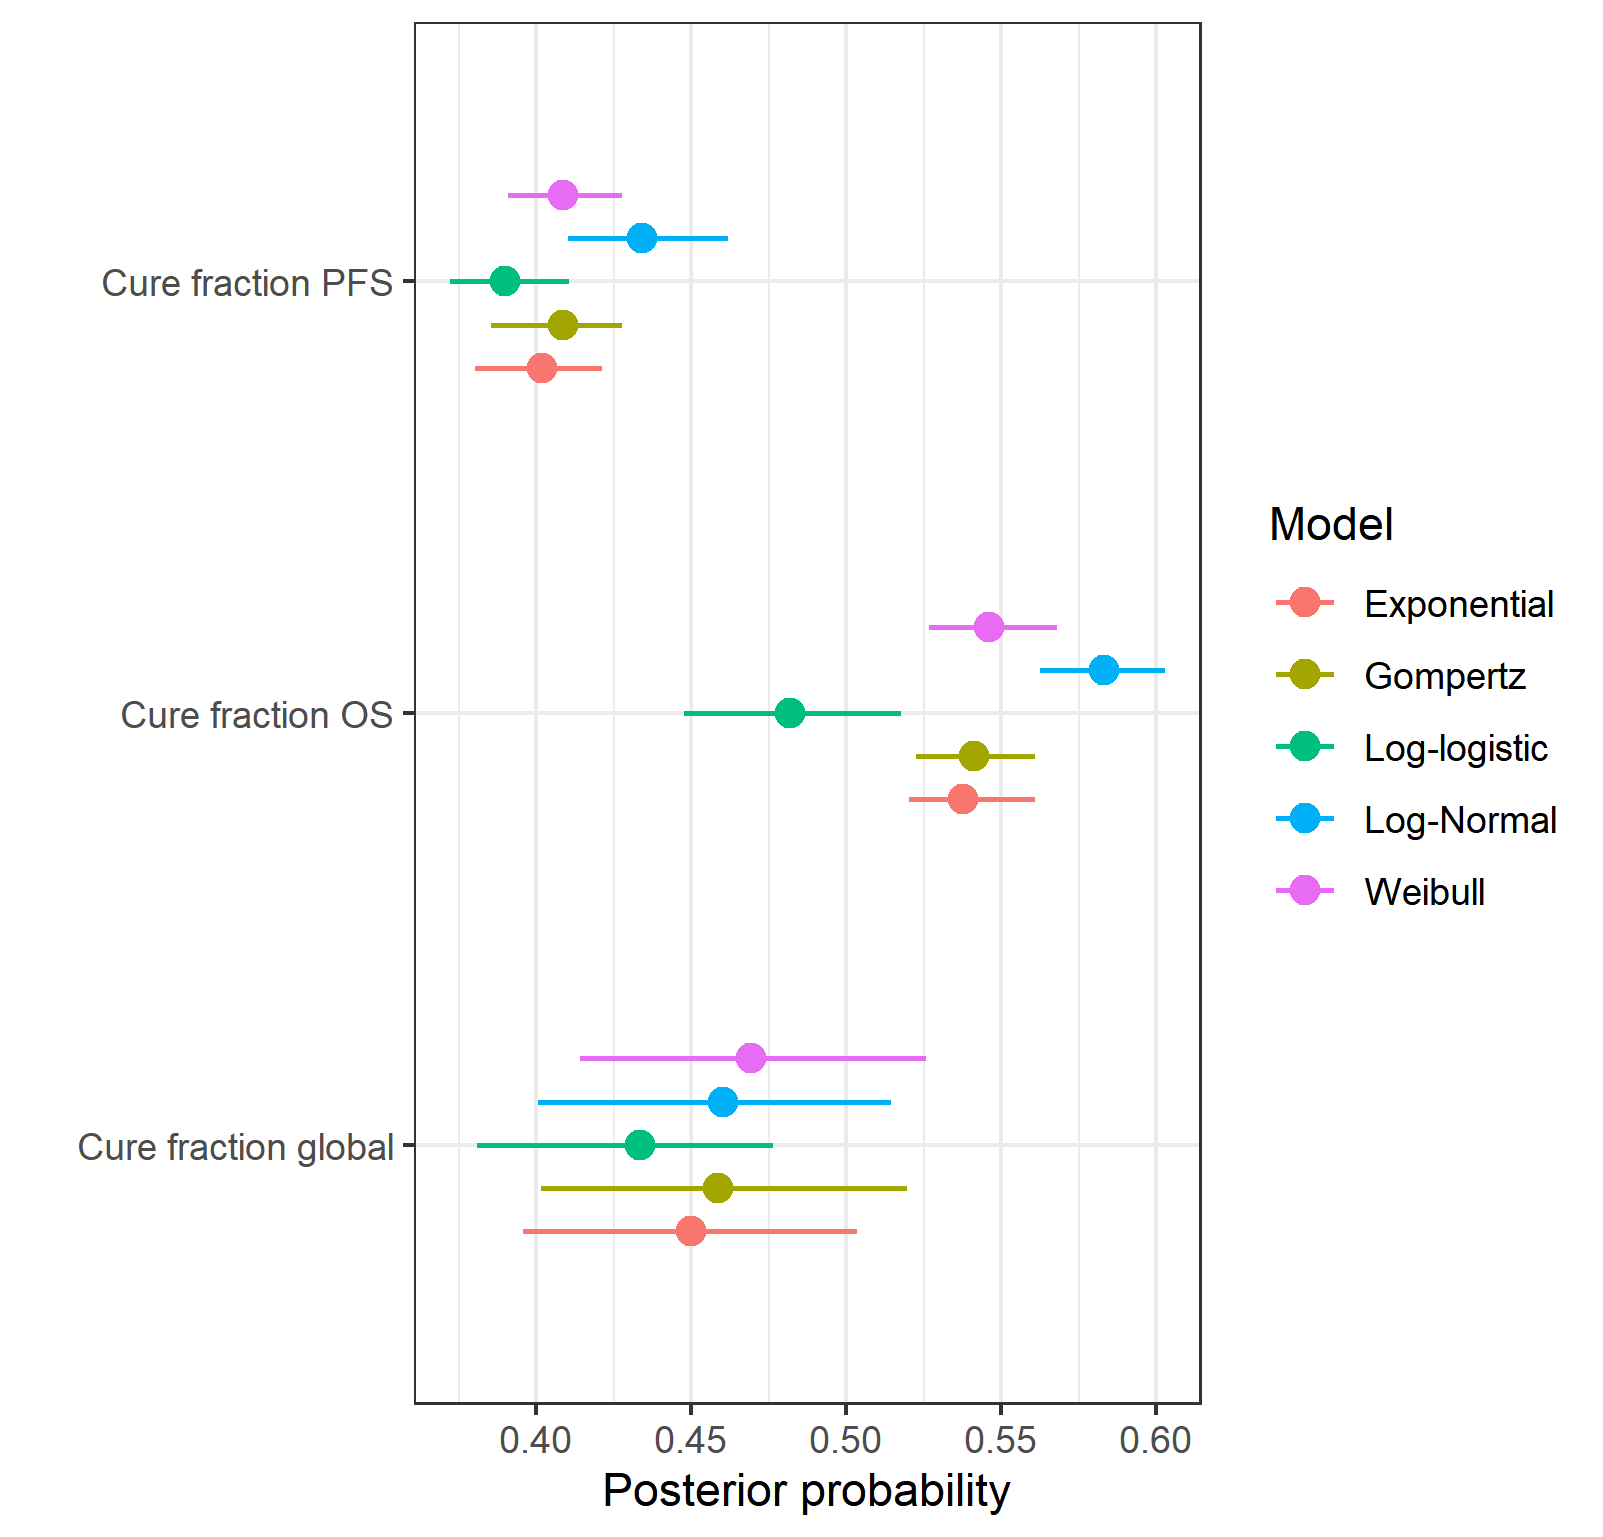
\includegraphics[width=0.6\linewidth]{../plots/cf hier_bg_fixed_hr1.63_forest_plot} 

}

\caption{\label{fig:forest_global_163}Forest plot of cure fraction posterior distributions for dual $ipilimumab$ and $nivolumab$ and background hazard ratio adjustment 1.63.}\label{fig:unnamed-chunk-15}
\end{figure}

The table below gives the leave-one-out cross validation statistics for
each model fit.

\begin{longtable}[]{@{}llllrr@{}}
\toprule
OS Distn & PFS Distn & Treatment & Statistic & Estimate &
SE\tabularnewline
\midrule
\endhead
exp & exp & NIVOLUMAB+IPILIMUMAB & elpd\_waic & -1548.19 &
53.04\tabularnewline
gompertz & gompertz & NIVOLUMAB+IPILIMUMAB & elpd\_waic.1 & -1548.57 &
53.21\tabularnewline
loglogistic & loglogistic & NIVOLUMAB+IPILIMUMAB & elpd\_waic.2 &
-1541.23 & 52.74\tabularnewline
lognormal & lognormal & NIVOLUMAB+IPILIMUMAB & elpd\_waic.3 & -1487.44 &
57.45\tabularnewline
weibull & weibull & NIVOLUMAB+IPILIMUMAB & elpd\_waic.4 & -1549.41 &
53.59\tabularnewline
exp & exp & NIVOLUMAB+IPILIMUMAB & p\_waic & 6.05 & 0.61\tabularnewline
gompertz & gompertz & NIVOLUMAB+IPILIMUMAB & p\_waic.1 & 6.59 &
0.53\tabularnewline
loglogistic & loglogistic & NIVOLUMAB+IPILIMUMAB & p\_waic.2 & 7.69 &
0.53\tabularnewline
lognormal & lognormal & NIVOLUMAB+IPILIMUMAB & p\_waic.3 & 14.76 &
1.22\tabularnewline
weibull & weibull & NIVOLUMAB+IPILIMUMAB & p\_waic.4 & 7.92 &
0.72\tabularnewline
exp & exp & NIVOLUMAB+IPILIMUMAB & waic & 3096.38 &
106.09\tabularnewline
gompertz & gompertz & NIVOLUMAB+IPILIMUMAB & waic.1 & 3097.14 &
106.41\tabularnewline
loglogistic & loglogistic & NIVOLUMAB+IPILIMUMAB & waic.2 & 3082.45 &
105.49\tabularnewline
lognormal & lognormal & NIVOLUMAB+IPILIMUMAB & waic.3 & 2974.89 &
114.90\tabularnewline
weibull & weibull & NIVOLUMAB+IPILIMUMAB & waic.4 & 3098.82 &
107.17\tabularnewline
\bottomrule
\end{longtable}

\hypertarget{references}{%
\subsection*{References}\label{references}}
\addcontentsline{toc}{subsection}{References}

\hypertarget{refs}{}
\begin{CSLReferences}{1}{0}
\leavevmode\hypertarget{ref-Amico2018}{}%
Amico, Maïlis, and Ingrid Van Keilegom. 2018. {``{Cure Models in
Survival Analysis}.''} \emph{Annual Review of Statistics and Its
Application} 5: 311--42.
\url{https://doi.org/10.1146/annurev-statistics-031017-100101}.

\leavevmode\hypertarget{ref-carpenter2017stan}{}%
Carpenter, Bob, Andrew Gelman, Matthew D Hoffman, Daniel Lee, Ben
Goodrich, Michael Betancourt, Marcus Brubaker, Jiqiang Guo, Peter Li,
and Allen Riddell. 2017. {``Stan: A Probabilistic Programming
Language.''} \emph{Journal of Statistical Software} 76 (1).

\leavevmode\hypertarget{ref-McElreath2018}{}%
McElreath, Richard. 2018. \emph{{Statistical Rethinking: A Bayesian
Course with Examples in R and Stan}}. Chapman and Hall/CRC.

\leavevmode\hypertarget{ref-Vehtari2017}{}%
Vehtari, Aki, Andrew Gelman, and Jonah Gabry. 2017. {``{Practical
Bayesian model evaluation using leave-one-out cross-validation and
WAIC}.''} \emph{Statistics and Computing} 27 (5): 1413--32.
\url{https://doi.org/10.1007/s11222-016-9696-4}.

\leavevmode\hypertarget{ref-wholifetables}{}%
WHO. 2020. {``{Life tables by country}.''}
\url{http://apps.who.int/gho/data/?theme=main\&vid=61160}.

\end{CSLReferences}

\end{document}
